% My Dell XPS has aspect ratio 1610 (16:10).
% Screen settings of the presentation room are 16:9. 
% Supported options are 32, 43, 54, 141, 149, 169, 1610, 2013
\documentclass[aspectratio=169, c]{beamer}
% \includeonlyframes{current}


\usetheme{CambridgeUS}
\usecolortheme{dolphin}

% Alter template settings after loading it with \usetheme
\setbeamertemplate{navigation symbols}{}
\setbeamertemplate{itemize item}{$\blacktriangleright$}
\setbeamertemplate{itemize subitem}{$\triangleright$}

% Override footnote
\makeatletter
\setbeamertemplate{footline}{%
\leavevmode%
\hbox{%
    \begin{beamercolorbox}[wd=.2\paperwidth,ht=2.25ex,dp=1ex,center]{author in head/foot}%
        \usebeamerfont{author in head/foot} Software Science % \insertshortauthor\expandafter\beamer@ifempty\expandafter{\beamer@shortinstitute}{}{~~(\insertshortinstitute)}
    \end{beamercolorbox}%
    \begin{beamercolorbox}[wd=.6\paperwidth,ht=2.25ex,dp=1ex,center]{title in head/foot}%
        \usebeamerfont{title in head/foot}\insertshorttitle
    \end{beamercolorbox}%
    \begin{beamercolorbox}[wd=.2\paperwidth,ht=2.25ex,dp=1ex,right]{date in head/foot}%
        \usebeamerfont{date in head/foot}\insertshortdate{}\hspace*{2em}
        \textcolor{darkgray}{\insertframenumber{}} \hspace*{2ex} 
    \end{beamercolorbox}}%
    \vskip0pt%
}
\makeatother


% Load packages
\usepackage{amssymb}
\usepackage{amsmath}
\usepackage{bussproofs}
\usepackage{color,soul}
\makeatletter
\let\UL\ul
\renewcommand\ul{\let\set@color\beamerorig@set@color \let\reset@color\beamerorig@reset@color \UL}
\makeatother

\newcommand{\mypos}[2]{\tikz[remember picture,baseline=(#2.base)]{\node[inner sep=0pt, anchor=base](#2){#1};}}

\usepackage[style=authortitle]{biblatex}
\addbibresource{../thesis/bibliography.bib}
\DeclareFieldFormat{bibhypertarget}{#1}

\usepackage[perpage]{footmisc}
\renewcommand{\thefootnote}{\arabic{footnote}}  % Use numeric symbols for footnotes

\definecolor{ao}{rgb}{0.0, 0.5, 0.0}

\newcommand{\speechthis}[2]{
    \tikz[remember picture,baseline]{\node[anchor=base,inner sep=0,outer sep=0]%
    (#1) {\underline{#1}};\node[overlay,ellipse callout,fill=blue!50] 
    at ($(#1.north)+(-.5cm,0.8cm)$) {#2};}%
}%

\usepackage{tikz}
\usetikzlibrary{arrows.meta, calc, decorations.pathmorphing, decorations.pathreplacing, shapes.arrows,shapes.multipart,chains,patterns, quotes,tikzmark, trees, positioning}


\usepackage[newfloat]{minted}
\usepackage{mathtools}
\usepackage{marvosym}

\usepackage{pifont}

\usepackage{ulem}
\usepackage{varwidth}
\usepackage{wasysym}
\usepackage{xcolor}
\usepackage{xspace}

\usepackage{c-restrict-language}

% Custom commands
\def\eg{\textit{e.g.}\@\xspace}
\def\ie{\textit{i.e.}\@\xspace}
\def\etall{\textit{et al.}\@\xspace}

\def\cink{C-in-$\mathbb{K}\ $}
\def\cinkrestrict{\cink} %\textsubscript{restrict} 

\newcommand{\greentriangleright}[0]{\begingroup\color{green}\triangleright\endgroup}

\newcommand{\soutthick}[1]{%
    \renewcommand{\ULthickness}{1.4pt}%
       \sout{#1}%
    \renewcommand{\ULthickness}{.4pt}% Resetting to ulem default
}

\newcommand{\executionannotation}[2]{%
    {\centering
    \begin{minipage}{\textwidth}
    M:\\[4pt]
    \begin{tikzpicture}
    \node[rectangle,draw,align=left] (M) {#1};
    \end{tikzpicture}
    \end{minipage}

    \vspace*{5pt}

    \begin{minipage}{.37\textwidth}
    R:\\[4pt]
    #2
    \end{minipage}
    }
}

\newcommand{\cmark}{\ding{51}}%
\newcommand{\xmark}{\ding{55}}%

\setbeamerfont{footnote}{size=\tiny}

% Title page
\title{An operational semantics for the C99 restrict type qualifier}
\author{Ties Klappe}
\institute{Radboud University}
\date{May 7\textsuperscript{th} 2024}

\titlegraphic { 
\tikz[remember picture, overlay] {\node[anchor=south east] at (current page.south east)[yshift=\footheight] {
\includegraphics[height=1.25cm]{ru-logo.png}};}
}

\begin{document}

\setlength{\fboxsep}{0pt}

% Render title page
\frame{\titlepage}

% Motivating example
% An example https://godbolt.org/z/h4rv6Y6G9
\begin{frame}[fragile]
\raggedright
\frametitle{A motivating example}

\begin{itemize}
    \item \textbf{Aliasing}: different symbolic names refer to the same object
    \item \textbf{Pointee}: the object pointed to by a pointer
\end{itemize}

\leavevmode\\

\begin{minted}[escapeinside=||,mathescape=true,linenos,texcomments]{c}
int foo1(int* p, int* q) {   
    *p = 10;
    *q = 11;
    return *p; // if $p$ and $q$ do not alias, $*p$ must evaluate to $10$
               // if $p$ and $q$ alias, $*p$ must evaluate to $11$
}
\end{minted}

\end{frame}

\begin{frame}[fragile]
\raggedright
\frametitle{A motivating example}

\begin{itemize}
    \item \textbf{Restrict}: programmer-provided information to inform the compiler specific pointers do not alias under certain conditions
\end{itemize}

\leavevmode \\

\begin{minted}[escapeinside=||,mathescape=true,linenos,texcomments]{c}
// \colorbox{blue!20}{Programmer}: hi compiler! I promise you $p$ and $q$ will not alias
int foo2(int* |\colorbox{blue!20}{restrict}| p, int* |\colorbox{blue!20}{restrict}| q) {
    *p = 10;
    *q = 11;
    return *p; // if $p$ and $q$ do not alias, $*p$ must evaluate to $10$
               // if $p$ and $q$ alias, $*p$ must evaluate to $11$
}
\end{minted}

\begin{figure}
\centering
\begin{tikzpicture}
    \node (p) {\mintinline{c}{p}};
    \node[right of = p, draw, rectangle] (pointee-p) {$10$};

    \node[right of = pointee-p] (q) {\mintinline{c}{q}};
    \node[right of = q, draw, rectangle] (pointee-q) {$11$};

    \draw[->] (p) -- (pointee-p);
    \draw[->] (q) -- (pointee-q);
\end{tikzpicture}
\end{figure}

\end{frame}


\begin{frame}[fragile]
\raggedright
\frametitle{A motivating example}
\begin{minted}[escapeinside=||,mathescape=true,linenos,texcomments]{c}
// \colorbox{blue!20}{Programmer}: hi compiler! I promise you $p$ and $q$ will not alias
// \colorbox{orange!20}{Compiler}: nice! Thanks to this information, I optimized your code
int foo2_optimized(int* |\colorbox{blue!20}{restrict}| p, int* |\colorbox{blue!20}{restrict}| q) {   
    *p = 10;
    *q = 11;
    return |\colorbox{orange!20}{\soutthick{*p} 10}|;
}

\end{minted}

\begin{figure}
\centering
\begin{tikzpicture}
    \node (p) {\mintinline{c}{p}};
    \node[right of = p, draw, rectangle] (pointee-p) {$10$};

    \node[right of = pointee-p] (q) {\mintinline{c}{q}};
    \node[right of = q, draw, rectangle] (pointee-q) {$11$};

    \draw[->] (p) -- (pointee-p);
    \draw[->] (q) -- (pointee-q);
\end{tikzpicture}
\end{figure}

\end{frame}

\begin{frame}[fragile]
\raggedright
\frametitle{The promise can be broken}
\begin{minipage}{0.4\textwidth}
\begin{minted}[escapeinside=||,mathescape=true,texcomments]{c}
int foo1(int* p, int* q) {   
    *p = 10;
    *q = 11;
    return *p;
}
\end{minted}
\end{minipage}%
\begin{minipage}{0.6\textwidth}
\begin{minted}[escapeinside=||,mathescape=true,texcomments]{c}
int foo2(int* |\colorbox{blue!20}{restrict}| p, int* |\colorbox{blue!20}{restrict}| q) {   
    *p = 10;
    *q = 11;
    return |\colorbox{orange!20}{\soutthick{*p} 10}|;
}
\end{minted}
\end{minipage}

\pause

\begin{minted}[escapeinside=||,mathescape=true,linenos,texcomments]{c}
int main() {
    int x;
    printf("%d, %d\n", foo1(&x, &x), foo2(&x, &x));
}
\end{minted}

\begin{figure}
\centering
\begin{tikzpicture}
    \node (p) {\mintinline{c}{p,q}};
    \node[right of = p, draw, rectangle, fill=red!20] (pointee) {$11$};

    \draw[->] (p) -- (pointee);
\end{tikzpicture}
\end{figure}

\begin{itemize}
    \item Prints $11, 10$, \ie the optimized code has a different result than the original code
    \item Is the optimization incorrect?
\end{itemize}

\end{frame}




\begin{frame}
\frametitle{Undefined behavior}
\begin{itemize}
    \item The programmer \textbf{broke} the promise by making $p$ and $q$ alias
    \item This induces \textbf{undefined behavior (UB, \rsub)}
    \begin{itemize}
        \item The compiler may \textit{assume} a program is free of UB
        \item It does not need to consider such programs when justifying optimizations (\ie the introductory optimization is sound)
    \end{itemize}
    \item In this presentation we only consider UB induced by restrict, but many other kinds exist
    (uninitialized memory loads, signed integer overflow, out-of-bounds accesses, ...)
\end{itemize}

\end{frame}

\begin{frame}
\frametitle{Undefined behavior}
\begin{itemize}
    \item To understand what uses of restrict induce undefined behavior, one should consult the ISO standard
\end{itemize}
\end{frame}

\begin{frame}
\frametitle{\textbf{6.7.3.1 Formal definition of} \texttt{restrict}}
\begin{figure}
\centering
{
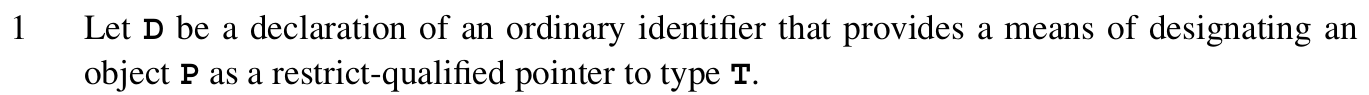
\includegraphics[width=0.9\textwidth]{restrict-definition-1.png}
}
{
\\
\qquad \vdots
\\
}
{
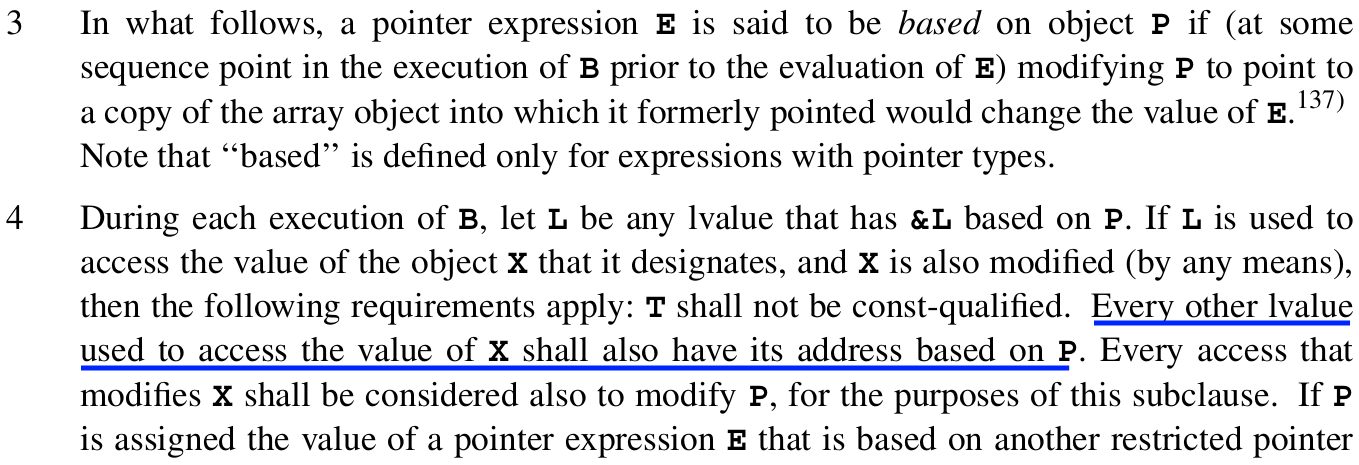
\includegraphics[width=0.9\textwidth]{restrict-definition-3-4-annotation-defined.png}
}
{
\\
\qquad \vdots
}
\end{figure}
\end{frame}

\begin{frame}
    \frametitle{\textbf{6.7.3.1 Formal definition of} \texttt{restrict}}
\begin{minipage}{0.5\textwidth}
\begin{itemize}
    \item Four N-documents submitted since 2018
    \item \setulcolor{red}\ul{Gustedt (2024)}\footnotemark: ``By its title it is a promise (to provide a formal definition) but it is in fact very delicate mix up of semantic concepts that make it almost impossible to comprehend from the given text.'' 
    \item MacDonald \etall (2022, 2024)\footnotemark \ report a bug in the definition of ``based on''
\end{itemize}
\end{minipage}%
\begin{minipage}{0.5\textwidth}
\begin{figure}
\centering
{
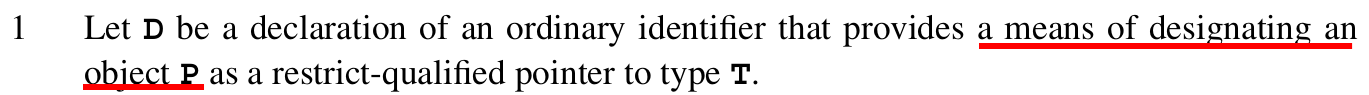
\includegraphics[width=0.95\textwidth]{restrict-definition-1-annotated.png}
}
{
\\
\qquad \vdots
\\
}
{
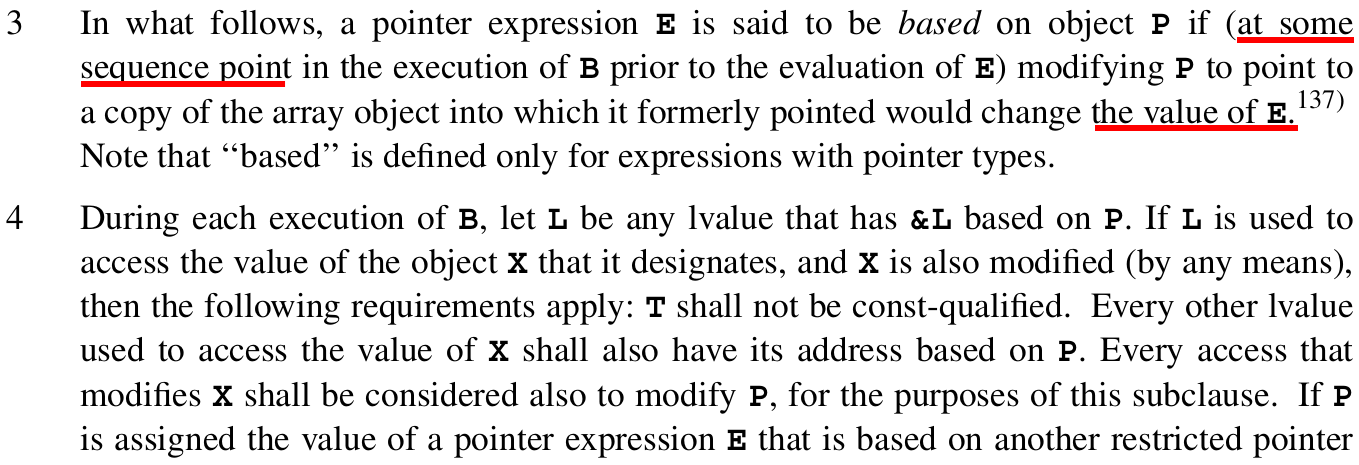
\includegraphics[width=0.95\textwidth]{restrict-definition-3-4-annotated.png}
}
{
\\
\qquad \vdots
}
\end{figure}
\end{minipage}

\footnotetext[1]{\cite{semanticsgustedt2024}}
\footnotetext[2]{\cite{defectmacdonald2022}} 

\end{frame}

\begin{frame}
\frametitle{Goals}

We want a definition for restrict which is: \\
\begin{enumerate}
    \item \textbf{Unambiguous}, \ie a formal semantics
    \item \textbf{Consistent} with the standard definition (to the extent possible) and/or existing compiler optimizations
    \item \textbf{Executable} such that one can test a program for UB 
    \item \textbf{Suitable} to be used for proving compiler optimizations correct (future work)
\end{enumerate}

\end{frame}

\begin{frame}
\frametitle{Approach (formal semantics)}

% \footcite{leroy2016compcert}\footcite{krebbers2015c}\footcite{memarian2023cerberus}
\begin{itemize}
    \item A vast landscape of formal semantics exists for C, \eg CompCert, CH\textsubscript{2}O and Cerberus
    \item Most of these projects have omitted restrict, except the executable \cink semantics
\end{itemize}

\pause
\begin{itemize}
    \item The paper\footcite{hathhorn2015defining} contains only a single paragraph on restrict, an extensive evaluation reveals several problems (2)
    \item As a rewrite-based semantics, it is not suitable for reasoning about optimization correctness à la CompCert (4)
    \begin{figure}
        \centering
    
    \begin{enumerate}
        \item \textcolor{ao}{Unambiguous: \cmark}
        \item \textcolor{red!80}{Consistent: \xmark}
        \item \textcolor{ao}{Executable: \cmark}
        \item \textcolor{orange!80}{Suitable: \raisebox{-0.5ex}{\scalebox{1.3}{!}}}
    \end{enumerate}
\end{figure}
\end{itemize}


\end{frame}


\begin{frame}
\frametitle{Contributions}
\centering
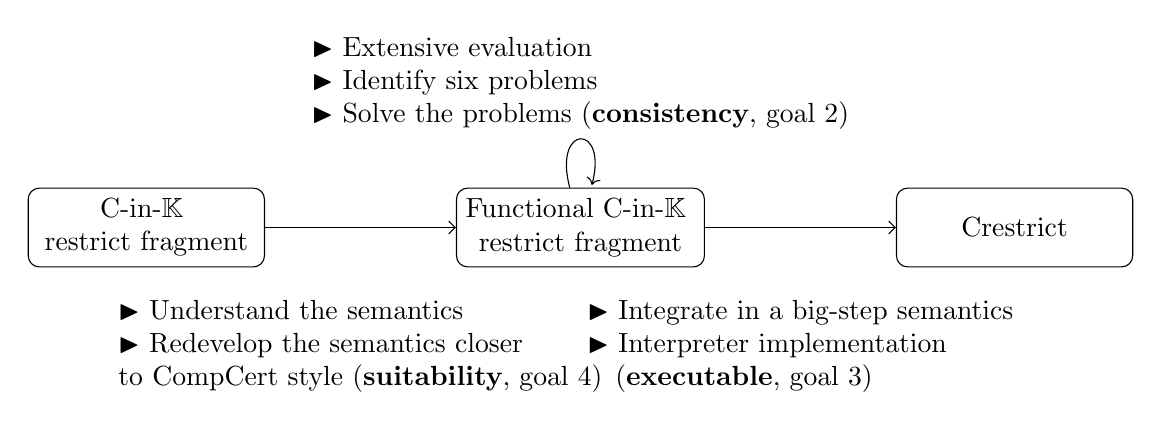
\begin{tikzpicture}[
    node distance=0.2\textwidth,
    artifact/.style={rectangle, rounded corners, minimum width=3cm, minimum height=1cm,text centered, draw=black,align=center}]

\node[artifact] (cink) {\cink\\restrict fragment};
\node[artifact, right = of cink] (cinkfunctional) {Functional \cink \\ restrict fragment};
\node[artifact, right = of cinkfunctional] (crestrict) {Crestrict};

\draw[-Straight Barb] (cink) -- (cinkfunctional)  node[midway, below=0.8cm, align=left] {%
    $\blacktriangleright$ Understand the semantics \\
    $\blacktriangleright$ Redevelop the semantics closer \\ to CompCert style (\textbf{suitability}, goal 4)
};

\path[-Straight Barb] (cinkfunctional) edge[loop above] node[midway, above, align=left] {%
    $\blacktriangleright$ Extensive evaluation \\ 
    $\blacktriangleright$ Identify six problems \\
    $\blacktriangleright$ Solve the problems (\textbf{consistency}, goal 2)
} (cinkfunctional);

\draw[-Straight Barb] (cinkfunctional) -- (crestrict) node[midway, right=1cm, below=0.8cm, align=left] {%
    $\blacktriangleright$ Integrate in a big-step semantics \\
    $\blacktriangleright$ Interpreter implementation \\ \quad (\textbf{executable}, goal 3)
};

\end{tikzpicture}
\end{frame}



% Restrict definition
\begin{frame}
\frametitle{Restrict definition (simplified)}
\begin{itemize}
    % \item A type qualifier for \textbf{pointer types}, \eg \mintinline{c}{int* restrict p;}
    \item A pointer is ``based on'' a restrict pointer if it depends on its value: \\
        \mintinline[mathescape=true]{c}{int x; int* restrict p = &x; int* q = p; // $q$ is based on $p$}  
    \item A \textbf{promise} that a restrict qualified pointer and pointers ``based on" it will \textbf{not alias} with other pointers during the \textbf{scope} it is alive if:
            \begin{itemize}
                \item The pointer is used to \textbf{access} the object it points to
                \item The object pointed to is \textbf{modified} (by any means)
            \end{itemize}
    % \item The compiler performs more optimizations based on this information
\end{itemize}
\end{frame}


\chapter{The Crestrict language}\label{chapter:crestrict}
In chapter \ref{chapt:improved-semantics} we proposed several refinements for the \cink{} semantics.
To show how we integrate the refined semantics into a programming language,
this chapter presents the Crestrict language, a small C-like language which aims to
provide sufficiently many features for defining a relevant restrict semantics.
The language is based on CompCert's \textit{Clight} language,
which is one of the intermediate target languages of the verified CompCert compiler \cite{blazy2009mechanized}.

In section \ref{section:syntax} the syntax of the language is presented. 
In section \ref{section:semantics} the different kinds of evaluation judgments and operational semantics are presented. 
Section \ref{section:memory-operations} defines and explains the different kinds of memory operations.
Finally, section \ref{section:restrict-operations} defines and explains the operations on the \Restrictstack.

The semantics we present in this chapter has also been implemented in an interpreter to make it executable.
Section \ref{section:implementation} will elaborate on this implementation, but throughout this chapter we already mention some differences between the
operational semantics and the implementation.  
% Should we give example derivations?

% Section 4.1
\section{Syntax}\label{section:syntax}
The syntax of the language and semantic constructs are presented in figure \ref{figure:syntax}.
Extensions and changes compared to the Clight language are mostly based on the domains that were presented in chapter \ref{chapt:improved-semantics}. 

All expressions are annotated with their type, which is left implicit in this thesis.
Instead, \typeof{e} is used to refer to the type which annotates $e$.
This information is used by both overloaded operators (\eg $+$ works on both integers and pointers) and
special rules for restrict qualified lvalues, which will be explained later.

An expression is either in \textit{lvalue position} (at the left-hand side of the assignment operator) or \textit{rvalue position} (anywhere else).
The only expressions that may be placed in lvalue position are $\Idvar$ and $*e$, and every expression may be placed in rvalue position.
In our language, this is not enforced by the syntax but by the operational semantics (which will be explained later).
The interpreter \textit{does} check for this before interpreting the program, because the program is first type checked after elaboration.

Assignments $e_1 = e_2$ assign the evaluated rvalue $e_2$ to the evaluated lvalue $e_1$ and are included in the statements.
Furthermore, procedure and function calls are also part of the statements.
The for-loop notation $\mathsf{for}(s_1, e_2, s_3) \ s$ means that $s_1$ is executed at the beginning of the loop,
$e_2$ is the condition, $s_3$ is executed at the end of each loop iteration and $s$ is the body.
Dynamic memory allocations and deallocations via $\mathsf{malloc}$ and $\mathsf{free}$ are included as statements.

A complete \Type \ is composed of a \Simpletype \ $\tau$ \ and a \Typequalifier \ $\tau_q$.
The supported variable types are \Inttype \ (signed 32-bit integers), \Ptrtype \ (pointers to type $\tau$) and \Arraytype \ (arrays of element type $\tau$ and size $n$).
Furthermore, \Functiontype \ denotes function types with return type $\tau$ and parameter types $\tau^*$, and \Voidtype \ denotes the void type.
Three types of type qualifiers are distinguished: \Noqualifier \ means that the type is unqualified,
\Globalrestrictqualifier \ means that the type is restrict qualified within a global declaration
and \Restrictqualifier \ means the type is restrict qualified within a local declaration.
The distinction between global and local restrict qualifiers is made to be able to distinguish the restrict declaration scope,
which will become more apparent by the definition of \textcode{get\_restrict\_scope} which will be explained in the next section.
Function definitions $(\tau, \Dclvar_1, \Dclvar_2, s)$ denote a function with
parameter declarations $\Dclvar_1$, local variable declarations $\Dclvar_2$, function body $s$ 
and return type $\tau$.
All local variable declarations must occur at the start of the function.
Finally, a program is composed of a list of global variable declarations and a list of function definitions.
The identifier denoting the program entry point is fixed to \textcode{main}.
This means that if no function definition for main is given, the program will get stuck immediately (\ie the syntax does not enforce main to be defined).

Compared to Clight, floats, structs, unions, type casts, switch statements and do loops are the largest omitted features of the language.
The most important reason for this is that we want a small language to focus on how the restrict feature affects its semantics,
while being large enough to be able to write some realistic example programs. 

All domains related to locations and provenance have previously been introduced
in figure \ref{fig:cink-domains2} and are merely repeated here for completeness.

Expressions in rvalue position may result in three types of values: $\vint{n}$ (32-bit integer values 
$n$), $\ptr{l}$ (a pointer value of location $l$) and $\vundef$ which represents the value at a memory location
which is uninitialized.
The \texttt{NULL} pointer, represented in Clight by the value $(\vint{0})$, is not modelled.
The reason for this is that the interpreter checks type compatibility between the left and right-hand sides of the assignment operator (\ie
one cannot assign an integer value to a pointer type), and omitting the \texttt{NULL} pointer did not limit our flexibility in creating test programs.

As in Clight, statements are evaluated to an outcome $\Outcomevar$ based on the approach of Norrish \cite{norrish1998c} and Huisman and Jacobs \cite{huisman2000java}.
This can either be \onormal, indicating the next statement can be executed; \ocontinue, for executing the next iteration of the current loop;
\obreak, for leaving the current loop, and \oreturn \ / \oreturnv{v} for leaving a function (possibly with return value $v$).

The functions and variables are mapped to their memory locations by two environments.
The global environment \Globalsvar \ is defined as a record and associates function and global variable identifiers
to the memory blocks they are stored in, and also contains the function definitions.
The local environment \Envvar \ is constructed per function and associates its parameter 
and local variable declarations with memory blocks.
The memory model is based on CompCert's model \cite{leroy2012compcert}, in which each allocation
results in a different block reference $\Blockvar \in \Block$.
A memory instance \Memvar $\in \Mem$ associates block references with a record $\Memblockvar \in \Memblock$.
The upper bound \Memblockmemberhi \ denotes the highest offset (exclusive) which may be addressed (the lower bound cannot be configured unlike in Clight, and is treated as 0).
The boolean \Memblockmemberdyn \ tracks whether a block was dynamically allocated (by means of a call to $\mathsf{malloc}$)
in order to determine whether it may be freed by the program.
Finally, the third component \Memblockmembercontent \ associates block offsets with values.
The \Scopemap \ tracks which scopes are active at a certain point of the execution,
and its purpose has been explained in section \ref{sec:filtering-bases}.

Finally, the restrict related domains which have previously been
introduced and explained in figure \ref{fig:cink-domains2} are listed for completeness.

% \begin{figure*}
% \centering
% \begin{minipage}{0.5\linewidth}
% \centering
% \[
% \begin{array}{@{}l@{\quad}lr}
%   \text{$\Globalsvar \in \Globals$ \ :=} & \left\{
%   \begin{array}{l}
%     \Globalsmemberenv : \Id \rightharpoonup \Block, \\
%     \Globalsmemberdefs : \Block \rightharpoonup \Fundef
%   \end{array}
%   \right\}   
% \end{array}
% \]
% \end{minipage}
% \begin{minipage}{0.5\textwidth}
% \centering
% \[
% \begin{array}{@{}l@{\quad}lr}
%     \text{$\Memblock$ \ :=} & \left\{
%     \begin{array}{l}
%     \Memblockmemberhi: \Intdomain, \\
%     \Memblockmemberdyn : \Booldomain, \\
%     \Memblockmembercontent : \Offset \rightharpoonup \Val
%     \end{array}
%     \right\}   
% \end{array}
% \]
% \end{minipage}%
% \caption{$\Globals$ and $MemBlock$ record}
% \label{figure:globals}
% \end{figure*}

\newpage
% \enlargethispage{3cm}

\begin{figure}[H]
    \[\def\arraystretch{1.00}
    {
    \begin{array}{lrl}
\multicolumn{3}{l}{\hspace{-5pt}\textbf{Expressions and statements}} \\[4pt]
    \Idvar \in \Id      & :=        & \textdom{String}                    \\
    e \in \Expr         & \bnfdef   & \Idvar \ | \ n \ | \ \mathconstr{sizeof}(\tau) \ | \ op_1  \ e \ | \ e_1 \ op_2 \ e_2 \ | \ \mathbin{*e} \ | \ \&e \   \\
    op_1 \in \textdom{UnaryOp}    & \bnfdef   & \smallbm{!} \  | \ \smallbm{\sim} \ | \ \smallbm{{-}}            \\
    op_2 \in \textdom{BinaryOp}   & \bnfdef   & \smallbm{+} \  | \ \smallbm{-} \ | \ \smallbm{*} \ | \ \smallbm{/} \ | \ \smallbm{\%} \ | \ \smallbm{<<} \ | \ \smallbm{>>} \ | \ \smallbm{\&} \ | \ \smallbm{|} \ | \ \smallbm{\hat{}}  \ \\
                                  & |         & \ \smallbm{<}  \ | \ \smallbm{\leq} \ | \ \smallbm{>} \ | \ \smallbm{\geq} \ | \ \smallbm{==} \ | \ \smallbm{!=}     \\
    s \in \Statement    & \bnfdef   & \mathsf{skip}  \ | \ \mathsf{break} \ | \ \mathsf{continue} \ | \  \mathsf{return} \ \Optiontype{e}                                            \\
                            & |         & e_1 = e_2 \ | \ e_1 = e_2(e^*) \ | \ e(e^*) \ | \ s_1; s_2                                                    \\
                            & |         & \mathsf{if}(e) \ s_1 \ \mathsf{else} \ s_2  \ | \ \mathsf{while}(e) \ s  \ | \ \mathsf{for}(s_1, e_2, s_3) \ s                           \\
                            & |         & e_1 = \mathsf{malloc}(e_2)  \ | \ \mathsf{free}(e)                                          \\[6pt]
\multicolumn{3}{l}{\hspace{-5pt}\textbf{Locations and provenance}} \\[4pt]
    \Blockvar \in \Block, \delta \in \Offset    & :=        & \mathbb{Z}    \\
    \Scopeidvar \in \Scopeid                    & :=        & \mathbb{Z}    \\
    \Simplelocvar \in SimpleLoc             & :=        & \Block \times \Offset                 \\
    \Locvar \in \Loc                        & :=        & \Simpleloc \times \Set{\Base}         \\
    \Basevar \in \Base                      & :=        & \Loc \times \Scopeid                  \\
    \Basesvar \in \Bases                    & :=        & \Set{\Base}                           \\
    \Basesfamvar \in \Basesfam              & :=        & \Set{\Bases}                 \\[6pt]
\multicolumn{3}{l}{\hspace{-5pt}\textbf{Values, outcomes, types, functions and programs}} \\[4pt]
    \Valvar \in \Val                        & \bnfdef   & \vint{n} \ | \ \ptr{l} \ | \ \vundef  \\
    \Outcomevar \in \Outcome                            & \bnfdef   & \onormal  \ | \ \obreak \ | \ \ocontinue\ | \ \oreturn \ | \ \oreturnv{v} \\
  
    \textdom{st} \in \Simpletype            & \bnfdef   & \Inttype \ | \ \Ptrtype  \ | \  \Arraytype \ | \ \Functiontype \ | \ \Voidtype  \\
    \tau_q \in \Typequalifier               & \bnfdef   & \Noqualifier \ | \ \Restrictqualifier \ | \ \Globalrestrictqualifier \\
    \tau \in \Type                          & :=        & \Simpletype \times \Typequalifier       \\ 
    \Dclvar \in \Declarations               & :=        & \List{\Type \times \Id}                        \\
    \Fundefvar \in \textdom{FunDef}         & :=        & \Type \times \Declarations \times \Declarations \times \Statement \\ %\tau \ \Dclvar_1 \set{\Dclvar_2; s}      \\
    \Fundclvar \in \Fundeclarations         & :=        & \List{\Id \times \textdom{FunDef}} \\
    P \in \textdom{Program}                 & :=        & \Declarations \times \Fundeclarations   \\[6pt] % dcl; \textdom{fun\_dcl}^*; \mathtt{main} = id        \\    
\multicolumn{3}{l}{\hspace{-5pt}\textbf{Environments and state members}} \\[4pt]
    \Envvar \in \Env                        & :=        & \Id \rightharpoonup \Block                                                                  \\
    \text{$\Globalsvar \in \Globals$ } & := & \left\{
  \begin{array}{l}
    \Globalsmemberenv : \Id \rightharpoonup \Block, \Globalsmemberdefs : \Block \rightharpoonup \Fundef
  \end{array}
  \right\} \\
    \Memblockvar \in \Memblock                        & :=        &  \left\{
        \begin{array}{l}
        \Memblockmemberhi: \Intdomain, \Memblockmemberdyn : \Booldomain, \Memblockmembercontent : \Offset \rightharpoonup \Val
        \end{array}
        \right\} \\
    \Memvar \in \Mem                        & :=        & \Block \rightharpoonup \Memblock                           \\
    \Scopemapvar \in \Scopemap              & :=        & \Scopeid \to \Booldomain \\
    \Restrictstatevar \in \Restrictstate    & \bnfdef   & \onlyread{\Basesfamvar} \ | \ \restricted{\Basesvar} \ | \ \rsub \ | \ \bot                                \\
    \Restrictmapvar \in \Restrictmap        & :=        & \Simpleloc \to \Restrictstate  \\

    \Restrictstackvar \in \Restrictstack    & :=        &  List(\Scopeid \times \Restrictmap) \\

    \end{array}
    }
    \]
\vspace*{-0.3cm}
\caption{Syntax of language and semantic constructs}
\label{figure:syntax}
\end{figure}
\begin{figure}[htp]
    \centering
\[
\begin{array}{@{}l@{\quad}lr}
  \text{$\Statevar \in \State$ \ :=} & \left\{
  \begin{array}{l}
    \Memstatemember : \Mem, \\
    \Restrictstatemember : \Restrictstack, \\
    \Scopesstatemember : \Scopemap
  \end{array}
  \right\}   
\end{array}
\]
\vspace*{-0.3cm}
\caption{$\State$ record}
\label{figure:state}
\end{figure}



% Section 4.2
\section{Natural semantics}\label{section:semantics}
This section describes the semantics of the language as a \textit{big-step operational semantics},
meaning expressions and statements are directly related to their results.
This kind of semantics relates closely to the interpreter implementation.
As in the Clight language, most judgments are parametrized by the global environment \Globalsvar \ and the local environment \Envvar.
Secondly, most judgments also take a state \Statevar \ which is defined as a record composed of three fields for the memory, restrict stack and scope map
as shown in figure \ref{figure:state}.



\subsection{Evaluation judgments}
Below the different kinds of evaluation judgments are defined.
Every judgment relating a program construct to some other syntactic construct (explained below) is paired with state $\Statevar$.
The evaluation result of a program construct is paired with the updated state $\Statevar'$ (which resulted from executing the program construct).


\[
\begin{array}{rll}
    G,E\vdash & e, \Statevar \lval \Locvar, \Statevar'                & \text{evaluation of expressions in lvalue position} \\
    G,E\vdash & e, \Statevar \rval \Valvar, \Statevar'                & \text{evaluation of expressions in rvalue position} \\
    G,E\vdash & e^*, \Statevar \rval v^*, \Statevar'            & \text{evaluation of lists of expressions} \\
    G,E\vdash & s, \Statevar \Downarrow \Outcomevar,\Statevar'  & \text{evaluation of statements} \\
    G \vdash  & \Fundefvar(\Valvar^*), \Statevar \Downarrow \Valvar, \Statevar'                & \text{evaluation of function invocations} \\
    \vdash    & P \Downarrow n   & \text{evaluation of programs}
\end{array}
\]


Expressions in lvalue position are evaluated to locations $\Locvar$ and 
expressions in rvalue position are evaluated to values $\Valvar$.
Statements are evaluated to outcomes \Outcomevar,  which indicate how the execution ended:
\onormal \ when it completed normally, and \obreak, \ocontinue \ or \oreturn \ otherwise.
Compared to Clight the expressions are no longer pure as they possibly modify the restrict stack (they still do not change the memory).


The original Clight language distinguished between diverging programs and undefined behavior by Leroy and Grall's coinductive approach \cite{leroy2009coinductive}:
they have separate evaluation rules for terminating programs and programs which diverge.
Currently, they use a small-step semantics which also enables the semantics to make this distinction.
In our operational semantics we do not distinguish between diverging programs and undefined behavior.
However, the implemented interpreter does make this distinction as non-terminating programs will eventually lead to a stack overflow
and programs with undefined behavior terminate immediately upon detection, resulting in an error message.

There are several auxiliary functions that will be used in the inference rules, which are defined in figure \ref{figure:Auxiliary-functions}.
The \textcode{add\_prov} function adds a base to the set of bases of pointer values and is the identity function for other values. 
The function \textcode{get\_restrict\_scope} determines the declaration scope of a restrict qualified type,
given the type qualifier and current state.
The restrict declaration scope for globally restrict qualified variables is fixed to \scope{main} (due the associated restrict block previously
mentioned in section \ref{section:iso-definition}).
The function \textcode{by\_reference} defines whether a type has Clight access mode ``by reference'',
indicating that during lvalue conversion the address of the lvalue expression is returned as a pointer value.
Finally, the \textcode{sizeof} function states that all types occupy one memory cell, except the array type
(which occupies the amount of elements multiplied by the size of the element type).
This reflects that the memory model works on the granularity of values rather than bytes.
There are two auxiliary functions which are used in the inference rules and not defined in figure \ref{figure:Auxiliary-functions}.
These functions perform the evaluation of binary operations (\textcode{eval\_binop}) and unary operators (\textcode{eval\_unop}).
As most evaluations are straightforward, only a partial definition is given in figure \ref{figure:indication-of-eval-functions}.
The case for the logical not (!) operator is shown, as well as the overloaded $+$ and $\mathbin{==}$ operators.


\begin{figure}[h]
\begin{functioncode}{
\textcode{add\_prov}                                                  &   :           & \Val \rightarrow \Base \rightarrow \Val \\
\textcode{add\_prov} \ (\ptr{(\Simplelocvar, \Basesvar)}) \ \Basevar      & \triangleq    & \ptr{(\Simplelocvar, \Basesvar \cup \set{\Basevar})} \\
\textcode{add\_prov} \ \Valvar \ \_                                   & \triangleq    & \Valvar \\~\\

\scope{main}                                                            &   :           & \Scopeid \\
\scope{main}                                                            & \triangleq    & 0 \\~\\

\textcode{get\_restrict\_scope}                                        &   :           & \Type \rightarrow \State \rightarrow \Optiontype{\Scopeid} \\
\textcode{get\_restrict\_scope} \ (\_, \Noqualifier) \ \_              & \triangleq    & \epsilon \\
\textcode{get\_restrict\_scope} \ (\_, \Globalrestrictqualifier) \ \_  & \triangleq    & \scope{main} \\
\textcode{get\_restrict\_scope} \ (\_, \Restrictqualifier) \ \Statevar & \triangleq    & \pseudoif \pseudolet ((\Scopeidvar, \_) : \_) = \Statevar.\Restrictstatemember \ \pseudothen \Scopeidvar \ \pseudoelse \epsilon \\~\\

\textcode{by\_reference}                                                &   :           & \Type \rightarrow \Booldomain \\
\textcode{by\_reference} \ (\textdom{st}, \_)                           & \triangleq    & \textdom{st} = (\mathconstr{Array} \ \_ \ \_) \lor \textdom{st} = (\mathconstr{Function} \ \_ \ \_) \\~\\

\textcode{is\_restrict}                                                 &   :           & \Type \rightarrow \Booldomain \\
\textcode{is\_restrict} \ (\_, \tau_\textdom{q})                        & \triangleq    & \tau_\textdom{q} = \Restrictqualifier \lor \tau_\textdom{q} = \Globalrestrictqualifier \\~\\

\textcode{sizeof}                                                       &   :           & \Type \rightarrow \Intdomain \\
\textcode{sizeof} \ ((\mathconstr{Array} \ \tau \ n), \_)               & \triangleq    & n \times \textcode{sizeof}(\tau) \\
\textcode{sizeof} \ \_                                                  & \triangleq    & 1 \\~\\
}
\end{functioncode}
\caption{Auxiliary functions for expression and statement semantics}
\label{figure:Auxiliary-functions}
\end{figure}

\newpage

\subsection{Expressions}
The natural semantics of expressions are given in figure \ref{fig:natural-semantics-expressions}.
The first three rules are for expressions in lvalue position, which evaluate to a \Loc.
The rules \ruletarget{E-Id-Env} and \ruletarget{E-Id-Glob} describe that a variable identifier \Idvar \ evaluates to $((\Blockvar, 0), \emptyset)$ for the $\Blockvar$
associated with \Idvar \ in \Envvar \ or \Globalsvar, the offset 0 and the empty set of bases.
The rule \ruletarget{E-Deref} describes that the dereference expression $*e$ evaluates to the location \Locvar, given that $e$ evaluated to \ptr{\Locvar} by
rvalue evaluation (\ie only pointer values can be dereferenced). 

The rule \ruletarget{E-Sizeof} does something special: the result of the auxiliary \textcode{sizeof} 
function is multiplied by four.
As was previously explained, the granularity of the memory model is at value level, not at byte level.
In order to give a sensible value we therefore act as if every memory cell occupies four bytes, which is reflected by this multiplication.

The remaining rules are for expressions in rvalue position, which evaluate to a \Val.

There are three rules that are concerned with \textit{lvalue conversion}, the occurrence of an lvalue expression $e$
in rvalue position.
The first rule is \ruletarget{E-Lval-Conv} which is applied for integer and pointer types (\ie non reference types) that are not restrict qualified.
The lvalue is evaluated into a location, the value at that location is loaded from memory and used for the result of the lvalue conversion. 
The \ruletarget{E-Lval-Conv-Ref} handles the special case when $e$ is of type array or function.
The value resulting from this rule is a pointer to the location of $e$.
For example, when you pass an array variable as argument to a function the passed value becomes a pointer to
the first element of the array due to this rule.
The third rule, \ruletarget{E-Lval-Conv-Restrict}, makes a case distinction for the case where $e$ is restrict qualified.
Because only pointer types can be restrict qualified, loading from the location \Locvar \ will result in a pointer value $\Valvar$.
The call to $\mathtt{add\_prov}$ adds the base \Locvar \ with the restrict declaration scope to the value $\Valvar$.
This rule ensures that all lvalues derived from a restrict qualified object get the correct provenance,
because every time the pointer value of a restrict qualified pointer is \textit{used} this rule applies.
Use means that restrict qualified pointer expression \mintinline{c}{E} is evaluated as rvalue into the pointer value
(for which lvalue conversion must take place).
This happens either because the pointer expression is directly used for an access, \eg \mintinline{c}{*E},
or because the pointer expression is assigned to another pointer, \eg \mintinline{c}{int* p = E;}.  

The rules \ruletarget{E-UnaryOp} and \ruletarget{E-BinaryOp} show how unary and binary operations are evaluated.
For binary operations, we have chosen the evaluation order to be left-to-right (which is the same in Clight).
Finally, the rule \ruletarget{E-AddressOf} shows how the address of an expression results in a pointer value.

\begin{figure}[H]
\[
\begin{array}{c|c|c}
\tau            &   \Valvar     &   (\textcode{eval\_unop} \ ! \ \tau \ \Valvar) \\ \hline
\Inttype        &   \vint{0}    &   (n == 0) \ ? \ \vint{1} : \vint{0} \\
\end{array}
\]
\[
\begin{array}{c|c|c|c|c}
\tau_1          &   \tau_2      &   \Valvar_1                                   &   \Valvar_2                               &   (\textcode{eval\_binop} \ + \ \tau_1 \ \tau_2 \ \Valvar_1 \ \Valvar_2) \\ \hline
\Inttype        &   \Inttype    &   \vint{n_1}                                  &   \vint{n_2}                              &   \vint{(n1 + n2)} \\
\Ptrtype        &   \Inttype    &   \ptr{((\Blockvar, \delta), \Basesvar)}      &   \vint{n}                                &   \ptr{((\Blockvar, \delta + n \times (\textcode{sizeof} \ \tau)), \Basesvar)} \\
\Inttype        &   \Ptrtype    &   \vint{n}                                    &   \ptr{((\Blockvar, \delta), \Basesvar)}  &   \ptr{((\Blockvar, \delta + n \times (\textcode{sizeof} \ \tau)), \Basesvar)} \\ \hline
                &               &                                               &                                           &   (\textcode{eval\_binop} \ \mathbin{==} \ \tau_1 \ \tau_2 \ \Valvar_1 \ \Valvar_2) \\ \hline
\Inttype        &   \Inttype    &   \vint{n_1}                                  &   \vint{n_2}                              &   (n_1 \mathbin{==} n_2) \ ? \ \vint{1} :  \vint{0} \\
\Ptrtype        &   \Ptrtype    &   \ptr{(\Simplelocvar_1, \_)}                 &   \ptr{(\Simplelocvar_2, \_)}             &   (\Simplelocvar_1 \mathbin{==} \Simplelocvar_2) \ ? \ \vint{1} : \vint{0}
\end{array}
\]
\caption{Excerpt of \textcode{eval\_unop} and \textcode{eval\_binop} functions}
\label{figure:indication-of-eval-functions}
\end{figure}

\begin{figure}[htp]
Expressions in lvalue position:
\threesemanticrules
{E-Id-Env} % Id (local env E)
{
    \begin{mathprooftree}
        \AxiomC{$E(\Idvar) = b$}
        \UnaryInfC{$\GEJudgment \Idvar,\Statevar \lval ((b, 0), \emptyset), \Statevar$}
    \end{mathprooftree}
}
{E-Id-Glob} % Id (global env G)
{
    \begin{mathprooftree}
        \AxiomC{$\Idvar \not\in \mathtt{dom}(E)$}
        \AxiomC{$G.\Globalsmemberenv(\Idvar) = b$}
        \BinaryInfC{$\GEJudgment \Idvar,\Statevar \lval ((b, 0), \emptyset), \Statevar$}
    \end{mathprooftree}
}
{E-Deref} % Dereference
{
    \begin{mathprooftree}
    \AxiomC{$\GEJudgment e,\Statevar \rval \ptr{l}, \Statevar'$}
    \UnaryInfC{$\GEJudgment *e,\Statevar \lval l, \Statevar'$}
    \end{mathprooftree}
}

Expressions in rvalue position: \\
% Integer values
\twosemanticrules{E-Int}
{
    \begin{mathprooftree}
    \AxiomC{\emptyaxiom}
    \UnaryInfC{$\GEJudgment n,\Statevar \rval \vint{n}, \Statevar$}
    \end{mathprooftree}
}
% Lvalue in rvalue position (otherwise/scalar)
{E-Lval-Conv}
{
    \hspace*{-1cm}
    \begin{array}{cc}
    \GEJudgment e,\Statevar \lval \Locvar, \Statevar' & (\textcode{load} \ \Statevar' \ l) = (\Statevar'', v) \\
    \lnot(\textcode{by\_reference} \ \typeof{e}) & \lnot(\isrestrict{e}) \\
    \hline
    \multicolumn{2}{c}{\GEJudgment e,\Statevar \rval v, \Statevar''}
    \end{array}
}

\twosemanticrules
% Sizeof a type
{E-Sizeof}
{
    \begin{mathprooftree}
    \AxiomC{$\textcode{sizeof} \ \tau = n$}
    \UnaryInfC{$\GEJudgment \mathconstr{sizeof}(\tau), \Statevar \rval \vint{(n \times 4)}, \Statevar$}
    \end{mathprooftree}
}
% Lvalue in rvalue position (case array/function)
{E-Lval-Conv-Ref}
{
    \hspace*{-1cm}
    \begin{mathprooftree}
    \AxiomC{$\GEJudgment e,\Statevar \lval \Locvar, \Statevar'$}
    \AxiomC{\textcode{by\_reference} \typeof{e}}
    \BinaryInfC{$\GEJudgment e,\Statevar \rval \ptr{\Locvar}, \Statevar'$}
    \end{mathprooftree}
}

% Lvalue in rvalue position (otherwise/scalar and restrict)
\semanticrule{E-Lval-Conv-Restrict}
{
    \begin{array}{cc}
    \GEJudgment e,\Statevar \lval \Locvar, \Statevar' & (\textcode{load} \ \Statevar' \ \Locvar) = (\Statevar'', \Valvar) \\
    \isrestrict{e} & (\getrestrictscope{\typeof{e}}{\Statevar}) = \Scopeidvar \\
    \hline
    \multicolumn{2}{c}{\GEJudgment e,\Statevar \rval (\textcode{add\_prov} \ \Valvar \ (\Locvar, \Scopeidvar)), \Statevar''}
    \end{array}
}

% Unary operator
\twosemanticrules{E-UnaryOp}
{
    \begin{mathprooftree}
    \AxiomC{$\GEJudgment e_1,\Statevar \rval v_1, \Statevar'$}
    \AxiomC{$(\mathtt{eval\_unop} \ op_1 \ $\typeof{e_1}$ \ v_1 ) = v$}
    \BinaryInfC{$\GEJudgment (op_1 \ e_1), \Statevar \rval v, \Statevar'$}
    \end{mathprooftree}
}
{E-AddressOf}
{
    \begin{mathprooftree}
    \AxiomC{$\GEJudgment e, \Statevar \lval \Locvar, \Statevar'$}
    \UnaryInfC{$\GEJudgment \&e, \Statevar \rval \ptr{l}, \Statevar'$}
    \end{mathprooftree}
}

\semanticrule{E-BinaryOp}
{
    \begin{mathprooftree}
    \AxiomC{$\GEJudgment e_1, \Statevar \rval v_1, \Statevar'$}
    \AxiomC{$\GEJudgment e_2, \Statevar' \rval v_2, \Statevar''$}
    \AxiomC{$(\mathtt{eval\_binop} \ op_2 \ \typeof{e_1} \ \typeof{e_2} \ v_1  \ v_2 ) = v$}
    \TrinaryInfC{$\GEJudgment (e_1 \ op_2 \ e_2), \Statevar \rval v, \Statevar''$}
    \end{mathprooftree}
}

\caption{Natural semantics of expressions}
\label{fig:natural-semantics-expressions}
\end{figure}



\subsection{Statements}
The natural semantics of statements are given in figure \ref{figure:natural-semantics-statements} (everything except loops)
and figure \ref{figure:natural-semantics-statements-loops} (loops).

The first interesting rule is the assignment rule, \ruletarget{S-Assign}.
The expression on the left-hand side of the assignment operator is evaluated as expression in lvalue position, resulting in a location $\Locvar$.
The expression on the right-hand side of the assignment operator is evaluated as expression in rvalue position, resulting in a value $\Valvar$.
The \textcode{store} rule is then invoked to update the state accordingly.

The \ruletarget{S-Procedure} and \ruletarget{S-Call} rules denote the semantics for function calls.
The location of the function definition is retrieved by evaluating the function identifier to a pointer.
Then, the arguments of the function call are evaluated into a list of values.
Finally, the function definition is invoked.
In the case of \ruletarget{S-Call} the value resulting from the function invocation is saved at the
evaluated location of the left-hand side expression.

The \ruletarget{S-Malloc} rule is for dynamic allocations.
The evaluated location $e_1$ is assigned a pointer value to the freshly allocated memory object.
Analogously to \ruletarget{E-Sizeof}, the amount of bytes $n$ to be allocated is divided by four to adjust
for the granularity of the memory model, which is why $n$ is required to be a multiple of 4.
The rule also allows $n$ to be 0, in which case a block is reserved with upper bound 0 (\ie the pointer value cannot be dereferenced).

The \Outcomeupdate{}{} relation describes how the \Outcome \ \Outcomevar \ is updated when the loop is exited prematurely
through a \obreak \ or \oreturn \ outcome.

While loops are described by three rules: \ruletarget{S-While-False} is the
normal terminating case of the loop when the condition evaluates to false.
\ruletarget{S-While-Abort} is the premature abortion of the loop, through a return or break statement.
Finally, the iteration is described by \ruletarget{S-While-True}: the condition evaluates to 
true and the execution of the body had a \onormal \ or \ocontinue \ outcome.

For loops are described by four rules.
The \ruletarget{S-For-False}, \ruletarget{S-For-Abort} and \ruletarget{S-For-True}
are very much similar to the corresponding while rules.
The only different rule is  \ruletarget{S-For-Init}, which evaluates the initial
statement.

The natural semantics of function invocations and complete programs are given in figure \ref{figure:semantics-fun-invoc-programs}.
The auxiliary functions used in the inference rules are defined in figure \ref{figure:auxiliary-functions-fun-invocations-programs}.

A function invocation consists of a function definition $\Fundefvar$ and a list of argument values $\Valvar_\textdom{args}$.
Before executing the function body, the function \textcode{init\_invocation} allocates memory for the parameters and local variables
and binds the argument values to the corresponding memory locations.
The result is a modified state $\Statevar'$ in which a new restrict map is pushed onto $\Restrictstatemember$,
a new scope is set to active in $\Scopesstatemember$ and the memory changes are updated in $\Memstatemember$.
The auxiliary function \textcode{fresh} is used to create a new scope identifier, and specializes for the
case where no scopes are active yet.
As we require the function main to be function from which the program starts, this means the scope identifier
for main is always set to \scope{main} to correspond with the definition of \textcode{get\_restrict\_scope}.
Besides the updated state, a local environment \Envvar \ (for the duration of the function invocation)
and list of block references \textdom{bs} are returned.
After executing the body $s$, the outcome \Outcomevar \ and function return type $\tau$ must have a compatible return value $\Valvar_\textdom{res}$,
checked by $(\Outcomevar, \tau) \mathrel{\#} \Valvar_\textdom{res}$.
The result of the invocation is the value $\Valvar_\textdom{res}$ and a new state in which the local variables have been freed from the
memory, the restrict map is popped off the restrict stack and the scope identifier of the function scope is set to inactive in the scope map.

The execution of a complete program is done by constructing the \Globals \ environment \Globalsvar.
This allocates space for all global variables and functions, and also relates the block references where
functions are stored to function definitions. Then, the function definition of the identifier \textit{main} is retrieved,
and invoked under the empty set \textcode{init\_state}.
The result is a number $n$, indicating the success status.


\begin{figure}[htp]
% Skip
\threesemanticrules{S-Skip}
{
    \begin{mathprooftree}
    \AxiomC{\emptyaxiom}
    \UnaryInfC{$\GEJudgment \mathconstr{skip}, \Statevar \Downarrow \onormal, \Statevar$}
    \end{mathprooftree}
}
% Break
{S-Break}
{
    \begin{mathprooftree}
    \AxiomC{\emptyaxiom}
    \UnaryInfC{$\GEJudgment \mathconstr{break}, \Statevar \Downarrow \obreak, \Statevar$}
    \end{mathprooftree}
}
% Continue
{S-Continue}
{
    \begin{mathprooftree}
    \AxiomC{\emptyaxiom}
    \UnaryInfC{$\GEJudgment \mathconstr{continue}, \Statevar \Downarrow \ocontinue, \Statevar$}
    \end{mathprooftree}
}
% Return void
\twosemanticrules{S-Return}
{
    \begin{mathprooftree}
    \AxiomC{\emptyaxiom}
    \UnaryInfC{$\GEJudgment (\mathconstr{return} \ \epsilon), \Statevar \Downarrow \oreturn, \Statevar$}
    \end{mathprooftree}
}
% Return val
{S-Return-Val}
{
    \begin{mathprooftree}
    \AxiomC{$G,E, \vdash e,\Statevar \rval v, \Statevar'$}
    \UnaryInfC{$\GEJudgment (\mathconstr{return} \ e), \Statevar \Downarrow \oreturnv{v}, \Statevar'$}
    \end{mathprooftree}
}

% Assignment (no restrict)
\semanticrule{S-Assign}
{
    \begin{mathprooftree}
    \AxiomC{$\GEJudgment e_1,\Statevar \lval l, \Statevar'$}
    \AxiomC{$\GEJudgment e_2,\Statevar' \rval v, \Statevar''$}
    \AxiomC{$(\textcode{store} \ \Statevar'' \ l \ v) = \Statevar'''$}
    \TrinaryInfC{$\GEJudgment (e_1 = e_2), \Statevar \Downarrow \onormal, \Statevar'''$}
    \end{mathprooftree}
}

% % Assignment (restrict)
% \semanticrule{S-Assign-Restrict}
% {   
%     \begin{array}{ccc}
%     \isrestrict{e_1} & \GEJudgment e_1,\Statevar \lval \Locvar, \Statevar' & \GEJudgment e_2,\Statevar' \rval \Valvar, \Statevar'' \\
%     \multicolumn{3}{c}{
%         \begin{array}{cc}
%             (\getrestrictscope{\typeof{e_1}}{\Statevar''}) = \Scopeidvar & (\textcode{store} \ \Statevar'' \ \Locvar \ (\textcode{add\_prov} \ \Valvar \ (\Locvar, \Scopeidvar))) = \Statevar'''
%         \end{array}
%         } \\
%     \hline
%     \multicolumn{3}{c}{\GEJudgment (e_1 = e_2), \Statevar \Downarrow \mathconstr{Normal}, \Statevar'''}
%     \end{array}
% }

% Function call (no assignment)
\semanticrule{S-Procedure}
{
    \begin{array}{ccc}
    \GEJudgment \Efunvar, \Statevar \rval \ptr{((b, 0),\emptyset)}, \Statevar' & \Globalsvar.\Globalsmemberdefs(b) = \Fundefvar & (\textcode{type\_of\_fundef} \ \Fundefvar) = \typeof{\Efunvar} \\
    \multicolumn{3}{c}{\begin{array}{cc}
        \GEJudgment \Eargvar, \Statevar' \rval \Vargvar, \Statevar'' & G \vdash \Fundefvar(\Vargvar),\Statevar'' \Downarrow \_, \Statevar'''
    \end{array}} \\
    \hline
    \multicolumn{3}{c}{\GEJudgment \Efunvar(\Eargvar), \Statevar \Downarrow \onormal, \Statevar'''}
    \end{array}
}

\semanticrule{S-Call}
{
    \begin{array}{ccc}
    \GEJudgment e, \Statevar \lval \Locvar, \Statevar'  & \GEJudgment \Efunvar, \Statevar' \rval \ptr{((b, 0),\emptyset)}, \Statevar'' & \Globalsvar.\Globalsmemberdefs(b) = \Fundefvar \\
    (\textcode{type\_of\_fundef} \ \Fundefvar) = \typeof{\Efunvar} & \GEJudgment \Eargvar, \Statevar'' \rval \Vargvar, \Statevar''' & G \vdash \Fundefvar(\Vargvar),\Statevar''' \Downarrow \Valvar, \Statevar'''' \\
    \multicolumn{3}{c}{(\textcode{store} \ \Statevar'''' \ l \ \Valvar) = \Statevar'''''} \\
    \hline
    \multicolumn{3}{c}{\GEJudgment e = \Efunvar(\Eargvar), \Statevar \Downarrow \onormal, \Statevar'''''}
    \end{array}
}

% Sequence (out s1 = Normal)
\semanticrule{S-Sequence}
{
    \begin{mathprooftree}
    \AxiomC{$\GEJudgment s_1,\Statevar \Downarrow \onormal, \Statevar'$}
    \AxiomC{$\GEJudgment s_2,\Statevar' \Downarrow \Outcomevar,\Statevar''$}
    \BinaryInfC{$\GEJudgment (s_1;s_2),\Statevar \Downarrow \Outcomevar, \Statevar''$}
    \end{mathprooftree}
}

% Sequence (out s1 != Normal)
\semanticrule{S-Sequence-Abort}
{
    \begin{mathprooftree}
    \AxiomC{$\GEJudgment s_1,\Statevar \Downarrow \Outcomevar, \Statevar'$}
    \AxiomC{$\Outcomevar \neq \onormal$}
    \BinaryInfC{$\GEJudgment (s_1;s_2),\Statevar \Downarrow \Outcomevar, \Statevar'$}
    \end{mathprooftree}
}

% Malloc (no restrict)
\semanticrule{S-Malloc}
{
    \begin{array}{cc}
    \GEJudgment e_1, \Statevar \lval l, \Statevar' & \GEJudgment e_2, \Statevar' \rval \vint{n}, \Statevar'' \\
    n \geq 0 \land (n \mathrel{\%} 4) = 0 & (\textcode{alloc} \ \Statevar'' \ (n / 4) \ \true) = (\Statevar''', \Blockvar) \\ 
   \multicolumn{2}{c}{(\textcode{store} \ \Statevar''' \ l \ (\ptr{((\Blockvar, 0), \emptyset)})) = \Statevar''''} \\
    \hline
    \multicolumn{2}{c}{\GEJudgment e_1 = \mathconstr{malloc}(e_2), \Statevar \Downarrow \onormal, \Statevar''''}
    \end{array}
}

% % Malloc (restrict)
% \semanticrule{S-Malloc-Restrict}
% {
%     \begin{array}{ccc}
%     \isrestrict{e_1} & \GEJudgment e_1, \Statevar \lval \Locvar, \Statevar' & \GEJudgment e_2, \Statevar' \rval \vint{n}, \Statevar'' \\
%     n \geq 0 \land (n \mathrel{\%} 4) = 0 & (\textcode{alloc} \ \Statevar'' \ (n / 4) \ \true ) = (\Statevar''', \Blockvar) &  (\getrestrictscope{\typeof{e_1}}{\Statevar'''}) = \Scopeidvar \\
%     \multicolumn{3}{c}{(\textcode{store} \ \Statevar''' \ \Locvar \ (\ptr{((\Blockvar, 0), \set{(\Locvar, \Scopeidvar)})})) = \Statevar''''} \\
%     \hline
%     \multicolumn{3}{c}{\GEJudgment e_1 = \mathconstr{malloc}(e_2), \Statevar \Downarrow \mathconstr{Normal}, \Statevar''''}
%     \end{array}
% }

% Free
\semanticrule{S-Free}
{
    \begin{mathprooftree}
    \AxiomC{$G, E \vdash e_1, \Statevar \lval \Locvar, \Statevar'$}
    \AxiomC{$\Statevar'.\Memstatemember(\textcode{block} \ \Locvar).\Memblockmemberdyn = \true$}
    \AxiomC{$(\textcode{free} \ \Statevar' \ \Locvar) = \Statevar''$}
    \TrinaryInfC{$\GEJudgment \mathconstr{free}(e_1), \Statevar \Downarrow \onormal, \Statevar''$}
    \end{mathprooftree}
}

\caption{Natural semantics of statements}
\label{figure:natural-semantics-statements}
\end{figure}

\newpage

\begin{figure}[htp]
\raggedright
\noindent Updates of statement outcomes: \\[4pt]
\centering
\Outcomeupdate{\obreak}{\onormal} \qquad \Outcomeupdate{\oreturn}{\oreturn} \qquad \Outcomeupdate{\oreturnv{v}}{\oreturnv{v}}
\\~\\

\raggedright While loops: \\[1pt]
\twosemanticrules{S-While-False}
{
    \begin{mathprooftree}
    \AxiomC{$\GEJudgment e, \Statevar \rval \Valvar, \Statevar'$}
    \AxiomC{$\textcode{is\_false} \ \Valvar$}
    \BinaryInfC{$\GEJudgment (\mathconstr{while}(e) \ s), \Statevar \Downarrow \onormal, \Statevar'$}
    \end{mathprooftree}
}
{S-While-Abort}
{
    \begin{array}{cc}
    \GEJudgment e, \Statevar \rval \Valvar, \Statevar' & \textcode{is\_true} \ \Valvar \\
    \GEJudgment s, \Statevar' \Downarrow \Outcomevar, \Statevar'' & \Outcomeupdate{\Outcomevar}{\Outcomevar'} \\
    \hline
    \multicolumn{2}{c}{\GEJudgment (\mathconstr{while}(e) \ s), \Statevar \Downarrow \Outcomevar', \Statevar''}
    \end{array}
}

\semanticrule{S-While-True}
{
    \begin{array}{cc}
    \GEJudgment e, \Statevar \rval \Valvar, \Statevar' & \textcode{is\_true} \ \Valvar \\
    \GEJudgment s, \Statevar' \Downarrow (\onormal | \ocontinue), \Statevar'' & \GEJudgment (\mathconstr{while}(e) \ s), \Statevar'' \Downarrow \Outcomevar, \Statevar''' \\
    \hline
    \multicolumn{2}{c}{\GEJudgment (\mathconstr{while}(e) \ s), \Statevar \Downarrow \Outcomevar, \Statevar'''}
    \end{array}
}
\\
\raggedright For loops:
\vspace*{-4pt}
\semanticrule{S-For-Init}
{
    \begin{mathprooftree}
    \AxiomC{$s_1 \neq \mathconstr{skip}$}
    \AxiomC{$\GEJudgment s_1,\Statevar \Downarrow \onormal, \Statevar'$}
    \AxiomC{$\GEJudgment (\mathconstr{for}(\mathconstr{skip}, e_2, s_3) \ s), \Statevar' \Downarrow \Outcomevar, \Statevar''$}
    \TrinaryInfC{$\GEJudgment (\mathconstr{for}(s_1, e_2, s_3) \ s), \Statevar \Downarrow \Outcomevar, \Statevar''$}
    \end{mathprooftree}
}


\twosemanticrules{S-For-False}
{
    \begin{mathprooftree}
    \AxiomC{$\GEJudgment e_2,\Statevar \rval \Valvar, \Statevar'$}
    \AxiomC{$\textcode{is\_false \ \Valvar}$}
    \BinaryInfC{$\GEJudgment (\mathconstr{for}(\mathconstr{skip}, e_2, s_3) \ s), \Statevar \Downarrow \onormal, \Statevar'$}
    \end{mathprooftree}
}
{S-For-Abort}
{
    \begin{array}{cc}
    \GEJudgment e_2, \Statevar \rval \Valvar, \Statevar' & \textcode{is\_true} \ \Valvar \\
    \GEJudgment s, \Statevar' \Downarrow \Outcomevar, \Statevar'' & \Outcomeupdate{\Outcomevar}{\Outcomevar'} \\
    \hline
    \multicolumn{2}{c}{\GEJudgment (\mathconstr{for}(\mathconstr{skip}, e_2, s_3) \ s), \Statevar \Downarrow \Outcomevar', \Statevar''}
    \end{array}
}
\semanticrule{S-For-True}
{
    \vspace*{-\baselineskip}
    \begin{array}{cc}
    \GEJudgment e_2, \Statevar \rval \Valvar, \Statevar' & \textcode{is\_true} \ \Valvar \\
    \GEJudgment s, \Statevar' \Downarrow (\onormal | \ocontinue, \Statevar'')  &   \GEJudgment s_3, \Statevar'' \Downarrow \onormal, \Statevar''' \\
    \multicolumn{2}{c}{\GEJudgment (\mathconstr{for}(\mathconstr{skip}, e_2, s_3) \ s), \Statevar''' \Downarrow \Outcomevar, \Statevar''''} \\
    \hline
    \multicolumn{2}{c}{\GEJudgment (\mathconstr{for}(\mathconstr{skip}, e_2, s_3) \ s), \Statevar \Downarrow \Outcomevar, \Statevar'''}
    \end{array}
}

\caption{Natural semantics of loops}
\label{figure:natural-semantics-statements-loops}
\end{figure}
\begin{figure}[H]
% Function invocation
\semanticrule{Fun-Invocation}
{
    \begin{array}{ccc}
    (\tau, \Dclvar_1, \Dclvar_2, s) = \Fundefvar  & (\textcode{init\_invocation} \ \Statevar \ \Dclvar_1 \ \Dclvar_2 \ \Valvar_\textdom{args}) = (\Statevar', \Envvar, \textdom{bs}) & \GEJudgment s,\Statevar' \Downarrow \Outcomevar,\Statevar'' \\
    (\Outcomevar, \tau) \mathrel{\#} v_\textdom{res} &  (\textcode{rmerge} \ \Statevar''.\Restrictstatemember \ \textdom{bs}) = R & (\textcode{free\_locals} \ \Statevar''.\Memstatemember \ \textdom{bs}) = M \\
    \multicolumn{3}{c}{\Statevar''' = [\Memstatemember := M, \Restrictstatemember := R, \Scopesstatemember := \Statevar''.\Scopesstatemember\set{\Scopeidvar \leftarrow \false}]} \\
    \hline
    \multicolumn{3}{c}{G \vdash \Fundefvar(\Valvar_\textdom{args}), \Statevar \Downarrow \Valvar_\textdom{res}, \Statevar'''}
    \end{array}
}

\end{figure}
% Programs
\begin{figure}[H]
\semanticrule{Program}
{
    \begin{array}{ccc}
    (\Dclvar, \Fundclvar) = P & \Statevar = \textcode{init\_state} & \Globalsvar = [\Globalsmemberenv := \emptyset, \Globalsmemberdefs := \emptyset] \\
    (\textcode{alloc\_globals} \ \Statevar \ \Globalsvar \ \Dclvar) = (\Statevar', \Globalsvar')  & & (\textcode{alloc\_fun\_defs} \ \Statevar' \ \Globalsvar' \ \Fundclvar) = (\Statevar'', \Globalsvar'') \\
    \Globalsvar''.\Globalsmemberenv(\textcode{``main"}) = \Blockvar  & \Globalsvar''.\Globalsmemberdefs(\Blockvar) = \Fundefvar  & \Globalsvar'' \vdash \Fundefvar(), \Statevar'' \Downarrow \vint{n}, \_ \\
    \hline
    \multicolumn{3}{c}{\vdash P \Downarrow n}
    \end{array}
}
\caption{Natural semantics of function invocations and programs}
\label{figure:semantics-fun-invoc-programs}
\end{figure}

\newpage

\begin{figure}[H]
\begin{functioncode}{
\textcode{(\#)}                                                 &   :           & (\Outcome \times \Type) \rightarrow \Val \rightarrow \Booldomain \\
(\onormal, \Voidtype) \mathrel{\#} \vundef                            &   \triangleq  & \true \\
(\oreturn, \Voidtype) \mathrel{\#} \vundef                            &   \triangleq  & \true \\
(\oreturn \ \Valvar, \tau) \mathrel{\#} \Valvar                        &   \triangleq  & \pseudoif \tau \neq \Voidtype \ \pseudothen \true \ \pseudoelse \false \\
\_ \mathrel{\#} \_                                                    &   \triangleq  & \false \\~\\

\textcode{fresh}                                                &   :           & \Scopemap \rightarrow (\Scopemap \times \Scopeid) \\
\textcode{fresh} \ \emptyset                                    &   \triangleq  & (\set{\scope{main} \mapsto \true}, \scope{main})  \\
\textcode{fresh} \ \Scopemapvar                                 &   \triangleq  & (\Scopemapvar\set{\Scopeidvar \leftarrow \true}, \Scopeidvar) \ \pseudowhere \Scopeidvar \not\in \textcode{dom}(\Scopemapvar) \\~\\

\textcode{deallocate}                                           &   :           &   \Mem \to \Block \to \Mem \\
\textcode{deallocate} \ \Memvar \ \Blockvar                     &   \triangleq  &   \Memvar\set{\Blockvar \leftarrow \Memvar(\Blockvar) \pseudowith [\Memblockmemberhi := 0]}\\~\\

\textcode{free\_locals}                                         &   :           &   \Mem \to \List{\Block} \to \Mem \\
\textcode{free\_locals} \ \Memvar \ []                          &   \triangleq  &   \Memvar \\
\textcode{free\_locals} \ \Memvar \ (\Blockvar : \textdom{bs})  &   \triangleq  &   (\textcode{free\_locals} \ (\textcode{deallocate} \ \Memvar \ \Blockvar) \ \textdom{bs}) \\~\\

\textcode{alloc\_vars}                                          &   :           & \State \rightarrow \Declarations \rightarrow \Optiontype{\State \times \Env \times \List{\Block}} \\
\textcode{alloc\_vars} \ \Statevar \ []                         &   \triangleq  & (\Statevar, [], []) \\
\textcode{alloc\_vars} \ \Statevar \ ((\tau, \Idvar) : \Dclvar) &   \triangleq  & \pseudolet (\Statevar', \Blockvar) = (\textcode{alloc} \ \Statevar \ (\textcode{sizeof} \ \tau) \ \false)\errbind \ \pseudoin \\
                                                                &               & \quad \pseudolet (\Statevar'', \Envvar, \textdom{bs}) = (\textcode{alloc\_vars} \ \Statevar' \ \Dclvar)\errbind \ \pseudoin \\
                                                                &               & \quad \quad (\Statevar'', \Envvar\set{\Idvar \leftarrow \Blockvar}, (b : \textdom{bs}) ) \\~\\

\textcode{bind\_params}                                         &   :           & \Mem \rightarrow \Env \rightarrow \Declarations \rightarrow \List{\Val} \rightarrow \Scopeid \rightarrow \Mem \\
\textcode{bind\_params} \ \Memvar \ \_ \ [] \ [] \ \_           &   \triangleq  & \Memvar \\
\textcode{bind\_params} \ \Memvar \ \Envvar \ ((\_, \Idvar) : \Dclvar) \ (\Valvar : \textdom{vs}) \ \Scopeidvar
                                                                &   \triangleq  & \pseudolet \Simplelocvar = (\Envvar(\Idvar) , 0) \ \pseudoin \\
                                                                &               & \quad \pseudoin (\textcode{bind\_params} \ \Memvar\set{\Simplelocvar \leftarrow \Valvar} \ \Envvar \ \Dclvar \ \textdom{vs} \ \Scopeidvar) \\~\\

\textcode{init\_invocation}                                     &   :           & \State \rightarrow \Declarations \rightarrow \Declarations \rightarrow \List{\Val} \rightarrow \\
                                                                &               & \Optiontype{\State \times \Env \times \List{\Block}} \\
\textcode{init\_invocation} \ \Statevar \ \Dclvar_1 \ \Dclvar_2 \ \Valvar_\textdom{args} \
                                                                &   \triangleq  & \pseudolet (\Statevar', \Envvar, \textdom{bs}) = (\textcode{alloc\_vars} \ \Statevar \ \Dclvar_1 + \Dclvar_2)\errbind \ \pseudoin \\
                                                                &               & \quad \pseudolet (\Scopemapvar, \Scopeidvar) = (\textcode{fresh} \ \Statevar'.\Scopesstatemember) \ \pseudoin \\
                                                                &               & \quad\quad \pseudolet \Memvar = (\textcode{bind\_params} \ \Statevar'.\Memstatemember \ \Envvar \ \Dclvar_1 \ \Valvar_\textdom{args} \ \Scopeidvar) \ \pseudoin \\
                                                                &               & \quad\quad\quad \pseudolet \Restrictstackvar = (\textcode{rnew} \ \Statevar'.\Restrictstatemember \ \Scopeidvar) \ \pseudoin \\ 
                                                                &               & \quad\quad\quad\quad ([\Memstatemember := \Memvar, \Restrictstatemember := \Restrictstackvar, \Scopesstatemember := \Scopemapvar], \Envvar, \textdom{bs}) \\~\\

\textcode{alloc\_globals}                                       &   :           & \State \rightarrow \Globals \rightarrow \Declarations \rightarrow \Optiontype{\State \times \Globals} \\
\textcode{alloc\_globals} \ \Statevar \ \Globalsvar \ []        &   \triangleq  & (\Statevar, \Globalsvar) \\
\textcode{alloc\_globals} \ \Statevar \ \Globalsvar \ (\tau, \Idvar) : \Dclvar
                                                                &   \triangleq  & \pseudolet (\Statevar', \Blockvar) = (\textcode{alloc} \ \Statevar \ (\textcode{sizeof} \ \tau) \ \false)\errbind \ \pseudoin \\
                                                                &               & \quad \pseudolet \Globalsvar' = \Globalsvar \pseudowith [\Globalsmemberenv := \Globalsvar.\Globalsmemberenv\set{\Idvar \leftarrow \Blockvar}] \ \pseudoin \\
                                                                &               & \quad \quad (\textcode{alloc\_globals} \ \Statevar' \ \Globalsvar' \ \Dclvar) \\~\\

\textcode{alloc\_fun\_defs}                                     &   :           & \State \rightarrow \Globals \rightarrow \Fundeclarations \rightarrow \Optiontype{\State \times \Globals} \\
\textcode{alloc\_fun\_defs} \ \Statevar \ \Globalsvar \ [] \         &   \triangleq  & (\Statevar, \Globalsvar) \\
\textcode{alloc\_fun\_defs} \ \Statevar \ \Globalsvar \ ((\Idvar, \Fundefvar) : \Fundclvar)
                                                                &   \triangleq  & \pseudolet (\Statevar', \Blockvar) = (\textcode{alloc} \ \Statevar \ 1 \ \false)\errbind \ \pseudoin \\
                                                                &               & \quad  \pseudolet \Globalsvar' = [\Globalsmemberenv := \Globalsvar.\Globalsmemberenv\set{\Idvar \leftarrow \Blockvar}, \Globalsmemberdefs := \Globalsvar.\Globalsmemberdefs\set{\Blockvar \leftarrow \Fundefvar}] \ \pseudoin \\
                                                                &               & \quad \quad (\textcode{alloc\_fun\_defs} \ \Statevar' \ \Globalsvar' \ \Fundclvar) \\~\\

\textcode{init\_state}                                          &   :           & \State \\
\textcode{init\_state}                                          &   \triangleq  & [\Memstatemember := \emptyset, \Restrictstatemember := [], \Scopesstatemember := \emptyset] \\~\\  

\textcode{is\_false}                                            &   :           & \Val \rightarrow \Booldomain \\
\textcode{is\_false} \ \Valvar                                  &   \triangleq  & \pseudoif \Valvar = (\vint{0}) \ \pseudothen \true \ \pseudoelse \false \\~\\

\textcode{is\_true}                                             &   :           & \Val \rightarrow \Booldomain \\
\textcode{is\_true} \ \Valvar                                   &   \triangleq  & \pseudoif \Valvar = \vundef \ \pseudothen \false \ \pseudoelse \lnot (\textcode{is\_false} \ \Valvar)


}
\end{functioncode}
\caption{Auxiliary functions for Crestrict function invocations, programs and loops}
\label{figure:auxiliary-functions-fun-invocations-programs}
\end{figure}

\newpage

% Section 4.3
\section{Memory operations}\label{section:memory-operations} %TODO: better name?
The memory operations, based on the CompCert memory model \cite{besson2015concrete}, are defined in figure \ref{figure:mem-operations}.
All memory operations are parametrized by a state \Statevar, whose updated variant is included in the return value in order to propagate modifications.
The memory instance \Memstatemember \ is directly modified by the operations, and the
restrict stack \Restrictstatemember \ indirectly by utilizing functions which operate on the \Restrictstack \ (section \ref{section:restrict-operations}).

Several specific notations are used in the definitions.
Location validity in the memory is defined by $\Memvar \validsym \Simplelocvar$, which denotes for some $\Simpleloc \ \Simplelocvar = (\Blockvar, \delta)$ that
\Blockvar \ is an allocated block and $\delta$ is a valid offset within the bounds of that block.
Given that a location \Simplelocvar \ is valid under a memory \Memvar, we know that
stores and loads of $\Memvar(\Simplelocvar)$ will not fail.
Hence, we will not explicitly check for failure at places where we use these operations when
location validity has been assured.
The function $\filterinactive$ filters out all bases with an inactive scope as was explained in section \ref{sec:filtering-bases}.
Finally, the access (\ie both loads and stores) $\Memvar(\Blockvar).\Memblockmembercontent(\delta)$ is abbreviated to $\Memvar((\Blockvar, \delta))$. 

Memory blocks are allocated through the \textcode{alloc} function, by providing the upper bound of the block capacity $n$ (the number of values
it must be able to store) and a boolean $d$ indicating whether the allocation is a \textit{dynamic} one (\ie from a call to \mathconstr{malloc}).
Tracking dynamic allocations is used to determine whether the program may free an object. %afaik they don't have this boolean.
All values of the block are initialized to \vundef.
The block identifier $b$ is always fresh and never gets reused.
The unspecified auxiliary function \textcode{new\_alloc\_id} simply uses the first unused block identifier (starting at 0 and increasing) 
and thus never fails in our implementation (but permits the possibility of failure for modelling limited memory storage).

When accessing a memory location via \textcode{load}, \textcode{store} or \textcode{free}, the first check is always whether the location
\Simplelocvar \ used for the access is valid by \Memvar \ \validsym \ \Simplelocvar.
Then, the restrict checks are applied by a call to the access-type specific function \textcode{rload}, \textcode{rstore} or \textcode{rfree},
which will be explained in section \ref{section:restrict-operations}.
These functions take as arguments the current restrict stack and a location whose bases are filtered by \filterinactive,
based on the active scope map at the time of the access.
The result is an optional \Restrictstack, in which the some case indicates that no restrict related rules were violated and the
value is the updated restrict stack. The none case represents that the program is assigned undefined behavior, \ie the access has led to
$\rsub$ somewhere in the restrict stack.

If no error has occurred, the \textcode{load} function retrieves the value from memory.
One additional check is performed to check whether the value does not equal \vundef, \ie the program does not load from uninitialized memory.
If this check is satisfied, a tuple of the updated state $\Statevar'$ and the retrieved value is returned.
Similarly, for the \textcode{store} function the value is stored and the updated memory instance is included in the returned state.
The \textcode{free} function only utilizes the \textcode{rfree} function for dynamically allocated locations (as these must be freed by the user).
Then, it simply sets the upper bound of the memory block to 0 by the auxiliary \textcode{deallocate} function, which indicates the block has been deallocated.

\begin{figure}[H]
\begin{functioncode}{
\textcode{alloc}                                                    &   :           &   \State \to \Intdomain \to \Booldomain \to \Optiontype{\State \times \Block} \\
\textcode{alloc} \ \Statevar \ n \ d \                              &   \triangleq  &   \pseudolet \Blockvar = (\textcode{new\_alloc\_id} \ \Statevar.\Memstatemember)\errbind \ \pseudoin (\Statevar', \Blockvar)  \\
                                                                    &               &   \quad \pseudowhere \Statevar' = \Statevar \pseudowith [\Memstatemember :=   \\
                                                                    &               &   \quad\quad \Statevar.\Memstatemember  \set{ \Blockvar \leftarrow [\Memblockmemberhi := n, \Memblockmemberdyn := d, \Memblockmembercontent := \setbuild{\delta \leftarrow \vundef}{\delta \in (0 \dots n)}] } \\
                                                                    &               &   \quad ] \\~\\
\textcode{load}                                                     &   :           &   \State \to \Loc \to \Optiontype{\State \times \Val} \\
\textcode{load} \ \Statevar \ (\Simplelocvar, \Basesvar)            &   \triangleq  &   \pseudoif \Statevar.\Memstatemember \validsym \Simplelocvar \ \pseudothen \\
                                                                    &               &   \quad \pseudolet \Restrictstackvar = (\textcode{rload} \ \Statevar.\Restrictstatemember \ (\Simplelocvar, (\filterinactive \ \Basesvar \ \Statevar.\Scopesstatemember))) \errbind \ \pseudoin \\
                                                                    &               &   \quad \quad \pseudolet \Valvar = \Statevar.\Memstatemember(\Simplelocvar) \ \pseudoin \\
                                                                    &               &   \quad \quad\quad \pseudoif \Valvar \neq \vundef \ \pseudothen (\Statevar', \Valvar) \\ 
                                                                    &               &   \quad \quad\quad\quad \pseudowhere \Statevar' = \Statevar \pseudowith [\Restrictstatemember := R] \\
                                                                    &               &   \quad \quad\quad \pseudoelse \nonesym \\
                                                                    &               &   \pseudoelse \nonesym \\~\\
\textcode{store}                                                    &   :           &   \State \to \Loc \to \Val \to \Optiontype{\State} \\
\textcode{store} \ \Statevar \ (\Simplelocvar, \Basesvar) \ \Valvar &   \triangleq  &   \pseudoif \Statevar.\Memstatemember \validsym \Simplelocvar \ \pseudothen \\
                                                                    &               &   \quad \pseudolet \Restrictstackvar = (\textcode{rstore} \ \Statevar.\Restrictstatemember \ (\Simplelocvar, (\filterinactive \ \Basesvar \ \Statevar.\Scopesstatemember)))\errbind \ \pseudoin \Statevar' \\
                                                                    &               &   \quad \quad \pseudowhere \Statevar' = \Statevar \pseudowith [ \\
                                                                    &               &   \quad \quad\quad \Memstatemember := \Statevar.\Memstatemember\set{\Simplelocvar \leftarrow \Valvar}, \\
                                                                    &               &   \quad \quad\quad \Restrictstatemember := \Restrictstackvar \\
                                                                    &               &   \quad \quad ] \\
                                                                    &               &   \pseudoelse \nonesym \\~\\
\textcode{free}                                                     &   :           &   \State \to \Loc \to \Optiontype{\State}  \\
\textcode{free} \ \Statevar \ (\Simplelocvar, \Basesvar)            &   \triangleq  &   \pseudoif \Statevar.\Memstatemember \validsym \Simplelocvar \ \pseudothen \\
                                                                    &               &   \quad \pseudolet \Restrictstackvar = \\
                                                                    &               &   \quad \quad \pseudoif \Statevar.\Memstatemember(\textcode{block} \ \Simplelocvar).\Memblockmemberdyn \ \pseudothen \\
                                                                    &               &   \quad \quad \quad (\textcode{rfree} \ \Statevar.\Restrictstatemember \ (\Simplelocvar, (\filterinactive \ \Basesvar \ \Statevar.\Scopesstatemember)))\errbind \\
                                                                    &               &   \quad \quad \pseudoelse \Statevar.\Restrictstatemember \\
                                                                    &               &   \quad \pseudoin \Statevar' \\ 
                                                                    &               &   \quad \quad \quad \pseudowhere \Statevar' = \Statevar \pseudowith [ \\
                                                                    &               &   \quad \quad \quad \quad \Memstatemember := (\textcode{deallocate} \ \Statevar.\Memstatemember \ (\textcode{block} \ \Simplelocvar)),\\
                                                                    &               &   \quad \quad \quad \quad \Restrictstatemember := R \\ 
                                                                    &               &   \quad \quad \quad ] \\
                                                                    &               &   \pseudoelse \nonesym \\~\\
\filterinactive                                                     &   :           &   \Bases \to \Scopemap \to \Bases \\
\filterinactive \ [] \ \_                                           & \triangleq    &   [] \\
\filterinactive \ (\Basevar : \Basesvar) \ \Scopemapvar
                                                                    & \triangleq    &   \pseudolet ((\Simplelocvar, \Basesvar'), \Scopeidvar) = \Basevar \ \pseudoin \\
                                                                    &               &   \quad \pseudoif \Scopemapvar(\Scopeidvar) = \true \ \pseudothen \\
                                                                    &               &   \quad \quad ((\Simplelocvar, (\filterinactive \ \Basesvar' \ \Scopemapvar)), \Scopeidvar) : (\filterinactive \ \Basesvar \ \Scopemapvar) \\
                                                                    &               &   \quad \pseudoelse \\ 
                                                                    &               &   \quad \quad \filterinactive \ \Basesvar \ \Scopemapvar 
}
\end{functioncode}
\caption{Memory operations over states \Statevar \ and auxiliary function \textcode{\filterinactive}}
\label{figure:mem-operations}
\end{figure}
    
\newpage

% Section 4,4
\section{Restrict stack operations}\label{section:restrict-operations}
This section presents the operations which transform the restrict stack and model the semantics of the restrict type qualifier.
The operations are based on the adaption of the functional style \cink{} semantics to accommodate the
Crestrict language (chapter \ref{chap:cink}) and the proposed refinements for the Crestrict semantics (chapter \ref{chapt:improved-semantics}).

All operations are parametrized by a restrict stack \Restrictstackvar, whose updated variant is included in the return value.
The operations are performed either when a memory location is accessed or when the scope changes.

When a new scope is invoked (by a function call), the \textcode{rnew} function is utilized to push a new tuple onto the restrict stack, 
composed of the passed \Scopeid \ and an empty \Restrictmap. Analogously, when a scope terminates (by a function return),
the function \textcode{rmerge} pops the \Restrictmap \ $\Restrictmapvar_m$ currently on top off the restrict stack.
The restrict states of all non-local locations which were modified (\ie which are in the domain of $\Restrictmapvar_m$)
are filtered and merged into the \Restrictmap \ $\Restrictmapvar_n$ which is now on top, if the restrict state of such a location is $\bot$.
If such a location has another state, a join was already performed by the \textcode{rcheck\_rec} rule, and the restrict state of the location within $\Restrictmapvar_m$ can simply be discarded.

The rules \textcode{rload} and \textcode{rstore} are invoked for load and store operations on the memory.
Both functions utilize the helper function \textcode{rcheck\_rec}, which performs the actual algorithm for checking undefined behavior
due to a memory access.
Basically, the algorithm always takes the map currently on top of the restrict stack, performs a join onto that map
with the restrict state representing the memory event and calls itself recursively onto the remaining restrict stack.
The recursive call represents the solution presented in section \ref{sec:moving-up-the-deferred-check}.
Whenever a join resulted in $\rsub$, the function returns $\epsilon$ immediately.
For the recursive call, the restrict state is filtered in order to remove bases with the scope identifier of the
scope which was popped off the restrict stack.
The function distinguishes between recursive calls: in the case of a recursive call the 
state is only joined if the current value does not equal $\bot$, as the restrict stack does not track until which scope 
a location is valid this prevents assigning a restrict state to locations in scopes in which it is no longer valid.

The \textcode{rstore} performs an additional \textcode{rmodify} operation, which takes as additional argument the bases
of the location used for the store.
This operation represents the solution presented in section \ref{subsec:modification-of-the-restrict-object}, which
updates the restrict state of the (possibly multiple) restrict qualified object(s) the location is derived from.

Finally, the \textcode{rfree} operation also updates the restrict stack if the operation was invoked by a call to free in the program
(for dynamically allocated memory locations only).
This allows the semantics to give undefined behavior for the program of section \ref{subsec:call-to-free}. 

\begin{figure}[H]
\begin{functioncode}{
        \textcode{rnew}                                         &   :           &   \Restrictstack \rightarrow \Scopeid \rightarrow \Restrictstack      \\
        \textcode{rnew} \ \Restrictstackvar \ \Scopeidvar \     &   \triangleq  &   (\Scopeidvar, \emptyset) : \Restrictstackvar \\~\\

        \textcode{rload}                                        &   :           &   \Restrictstack \rightarrow \Loc \rightarrow \Optiontype{\Restrictstack} \\
        \textcode{rload} \ \Restrictstackvar \ (\Simplelocvar, \Basesvar)
                                                                &   \triangleq  &   \pseudolet \Restrictstatevar = (\onlyread{\set{\Basesvar}}) \ \pseudoin (\textcode{rcheck\_rec} \ \Restrictstackvar \ \Restrictstatevar \ \Simplelocvar \ \false) \\~\\

        \textcode{rstore}                                       &   :           &   \Restrictstack \rightarrow \Loc \rightarrow \Optiontype{\Restrictstack} \\
        \textcode{rstore} \ \Restrictstackvar \ (\Simplelocvar, \Basesvar)
                                                                &   \triangleq  &   \pseudolet \Restrictstatevar = (\restricted{\Basesvar}) \ \pseudoin \\
                                                                &               &   \quad \pseudolet \Restrictstackvar' = (\textcode{rcheck\_rec} \ \Restrictstackvar \ \Restrictstatevar \ \Simplelocvar \ \false)\errbind \ \pseudoin \\
                                                                &               &   \quad \quad (\textcode{rmodify} \ \Restrictstackvar' \ \Basesvar) \\~\\ 

        \textcode{rmodify}                                      &   :           &   \Restrictstack \rightarrow \Bases \rightarrow \Optiontype{\Restrictstack} \\
        \textcode{rmodify} \ \Restrictstackvar \ \emptyset      &   \triangleq  &   \Restrictstackvar \\
        \textcode{rmodify} \ \Restrictstackvar \ ((\Locvar, \_) : \Basesvar)
                                                                &   \triangleq  &   \pseudolet \Restrictstackvar' = (\textcode{rstore} \ \Restrictstackvar \ \Locvar)\errbind \ \pseudoin (\textcode{rmodify} \ \Restrictstackvar' \ \Basesvar) \\~\\

        \textcode{rcheck\_rec}                                  &   :           &   \Restrictstack \rightarrow \Restrictstate \rightarrow \Simpleloc \rightarrow \Booldomain \rightarrow \\
                                                                &               & \Optiontype{\Restrictstack} \\
        \textcode{rcheck\_rec} \ [] \ \_ \ \_ \ \_                  &   \triangleq  &   [] \\  
        \textcode{rcheck\_rec} \
            (\Scopeidvar, \Restrictmapvar_\textdom{cur}) :
            \Restrictstackvar \ \Restrictstatevar \
            \Simplelocvar \ \textdom{rec}
                                                                &   \triangleq  &   \pseudolet \Restrictmapvar_\textdom{hd} = \\
                                                                &               &   \quad \pseudoif (\Restrictmapvar_{\textdom{cur}}(\Simplelocvar) = \bot) \land \textdom{rec} \ \pseudothen \\
                                                                &               &   \quad \quad (\Scopeidvar, \Restrictmapvar_{\textdom{cur}}) \\
                                                                &               &   \quad \pseudoelse \\
                                                                &               &   \quad \quad \pseudolet \Restrictstatevar_\textdom{new} = \Restrictstatevar \joinsym \Restrictmapvar_{\textdom{cur}}(\Simplelocvar) \ \pseudoin \\
                                                                &               &   \quad \quad \quad \pseudoif \Restrictstatevar_\textdom{new} \neq \rsub \ \pseudothen \\
                                                                &               &   \quad \quad \quad \quad (\Scopeidvar, \Restrictmapvar_{\textdom{cur}}\set{\Simplelocvar \leftarrow \Restrictstatevar_\textdom{new}}) \\
                                                                &               &   \quad \quad \quad \pseudoelse \epsilon \\
                                                                &               &   \pseudoin (\Restrictmapvar_\textdom{hd}\errbind : (\textcode{rcheck\_rec} \ \Restrictstackvar \ (\filterbases \ (\Restrictstatevar, \Scopeidvar)) \ \Simplelocvar \ \true)\errbind) \\~\\

        \textcode{rfree}                                        &   :           &   \Restrictstack \rightarrow \Loc \rightarrow \Optiontype{\Restrictstack} \\
        \textcode{rfree} \ \Restrictstackvar \ (\Simplelocvar, \Basesvar)
                                                                &   \triangleq  &   \pseudolet \Restrictstackvar' = (\textcode{rcheck\_rec} \ \Restrictstackvar \ (\restricted{\Basesvar}) \ \Simplelocvar \ \false)\errbind \ \pseudoin \\
                                                                &               &   \quad (\textcode{remove} \ \Restrictstackvar' \ \Simplelocvar) \\~\\

        \textcode{remove}                                       &   :           &   \Restrictstack \rightarrow \Simpleloc \rightarrow \Restrictstack \\
        \textcode{remove} \ [] \ \_                             & \triangleq    &   [] \\
        \textcode{remove} \ (\Restrictmapvar : \Restrictstackvar) \ \Simplelocvar
                                                                &   \triangleq  &   (\Restrictmapvar \setminus \set{(\Simplelocvar, \_)}) : (\textcode{remove} \ \Restrictstackvar \ \Simplelocvar) \\~\\

        \textcode{rmerge}                                       &   :           &   \Restrictstack \rightarrow \List{\Block} \rightarrow \Restrictstack \\
        \textcode{rmerge} \ [] \ \_                               &   \triangleq  &   [] \\
        \textcode{rmerge} \ (\_ : []) \ \_                          &   \triangleq  &   [] \\
        \textcode{rmerge} \ ((\Scopeidvar_m, \Restrictmapvar_m) : (\Scopeidvar_n, \Restrictmapvar_n) : \Restrictstackvar) \
                            \textdom{bls}                      &   \triangleq  &   \pseudolet \textdom{sls} = \setbuild{\Simplelocvar}{\Simplelocvar \in \textcode{dom}(\Restrictmapvar_m) \land \Simplelocvar \not\in \textdom{bls} \land \Restrictmapvar_n(\Simplelocvar) = \bot} \ \pseudoin \\
                                                                &               &   \quad \pseudolet \Restrictmapvar_o = \setbuild{\Simplelocvar \mapsto (\textcode{filter\_bases} \ (\Restrictmapvar_m(\Simplelocvar), \Scopeidvar_m))}{\Simplelocvar \in \textdom{sls}} \ \cup \\
                                                                &               &   \qquad\qquad\quad\;\;\, \setbuild{\Simplelocvar \mapsto \Restrictmapvar_n(\Simplelocvar)}{\Simplelocvar \in \textcode{dom}(\Restrictmapvar_n) \land  \Simplelocvar \not\in \textdom{sls}} \ \pseudoin \\
                                                                &               &   \quad \quad (\Scopeidvar_n, \Restrictmapvar_o) : R \\
}
\end{functioncode}
\caption{Restrict operations over restrict stacks \Restrictstackvar}
\label{figure:restrict-operations}
\end{figure}


% \newpage

% \subsection{Undefined behavior and restrict}

% Lemma: if program evaluates to a result value $n$ and state $\Statevar$, it does not contain UB.

% $P \Downarrow n, \Statevar \implies$ no \rsub in the values of $\Statevar.\Restrictstatemember$ 

% Eh, we dont have a restrict stack with values anymore.



\begin{frame}[fragile]
\frametitle{The \cinkrestrict semantics}
Two features are jointly used to support restrict:\\
\begin{enumerate}
    \item Pointer values have some extra information, called \textbf{\textcolor{blue}{bases}}
    \begin{itemize}
        \item Tracks on which restrict qualified pointer(s) a pointer is based
        \item Used to distinguish pointers to the same address
    \end{itemize}
    \vspace*{5pt}
    \[
    \begin{array}{lll}
    \Blockvar \in \Block, \Scopeidvar \in \Scopeid &  :=  & \Intdomain \\
    \Basesvar \in \Bases & := & \Set{\mypos{$\Block$}{cink-provenance-block} \times \mypos{$\Scopeid$}{cink-provenance-scope}} \\~\\
    \strut\Val  & \bnfdef   & \ptr{(\mypos{$\Block$}{cink-abstract-val} \times \textcolor{blue}{\Bases})} \ | \ ... 
    \end{array}
    \hspace{1000pt minus 1fill}
    \]

\pause

    \begin{tikzpicture}[overlay, remember picture]
    \draw[red!30] ([yshift=-2pt]cink-abstract-val.base east)--([yshift=-2pt]cink-abstract-val.base west) to[bend left=25] ++(-.75,-.25) node[red!60, anchor=east] {\footnotesize Address of the pointee};
    \draw[blue!30] ([yshift=-2pt]cink-provenance-block.base east)--([yshift=-2pt]cink-provenance-block.base west) to[bend left=25] ++(-.75, -.25) node[blue!60, anchor=east] {\footnotesize Address of restrict pointer};
    \draw[blue!30] ([yshift=-2pt]cink-provenance-scope.base west)--([yshift=-2pt]cink-provenance-scope.base east) to[bend right=25] ++(.75, -.25) node[blue!60, anchor=west] {\footnotesize Restrict pointer declaration scope};
    
    \end{tikzpicture}
\end{enumerate}

\end{frame}

\begin{frame}[fragile]
    \frametitle{The \cinkrestrict semantics}
    Two features are jointly used to support restrict:\\
    \begin{enumerate}
        \setcounter{enumi}{1}
        \item The \textbf{restrict stack} tracks what memory accesses are allowed by maintaining a per-location \textbf{restrict state}
    \end{enumerate}

    \[
    \begin{array}{lll}
    \Restrictstate  &   \bnfdef     & \mypos{$\onlyread{\Basesvar}$}{cink-stack-or} \ | \ \mypos{$\restricted{\Basesvar}$}{cink-stack-rs} \ | \ \mypos{$\unrestricted$}{cink-stack-un} \\~\\
    R \in \Restrictstack  & := & \List{\mypos{$\Scopeid$}{cink-stack-scope} \times (\Block \rightarrow \Restrictstate)}
    \end{array}
    \hspace{1000pt minus 1fill}
    \]

\pause

    \begin{tikzpicture}[overlay, remember picture]
    \draw[red!30] ([yshift=-2pt]cink-stack-or.base east)--([yshift=-2pt]cink-stack-or.base west) to[bend left=25] ++(-.75,-.25) node[red!60, align=left, anchor=east, yshift=-5pt] {\footnotesize Load via \ptr{(\_, \Basesvar)}};
    \draw[red!30] ([yshift=-2pt]cink-stack-rs.base east)--([yshift=-2pt]cink-stack-rs.base west) to[bend left=25] ++(-.5,-.25) node[red!60, align=left, anchor=center,yshift=-5pt] {\footnotesize Store via \ptr{(\_, \Basesvar)}};
    \draw[red!30] ([yshift=-2pt]cink-stack-un.base east)--([yshift=-2pt]cink-stack-un.base west) to[bend right=25] ++(.5,-.25) node[red!60, align=left, anchor=west,yshift=-5pt] {\footnotesize Loads via pointers with different bases};
    \draw[red!30] ([yshift=-2pt]cink-stack-scope.base west)--([yshift=-2pt]cink-stack-scope.base east) to[bend right=25] ++(.75,-.25) node[red!60, align=left, anchor=west] {\footnotesize Scope in which the access occured};
    \end{tikzpicture}

\end{frame}

\begin{frame}[fragile]
\frametitle{The introductory example under the \cinkrestrict semantics}
\begin{minted}[escapeinside=||,mathescape=true,texcomments]{c}
// Scope \scope{foo}
int foo(int* restrict p, int* restrict q) {   
    *p = 10;
    *q = 11;
    return *p;
}
\end{minted}

\begin{figure}[h]
\centering
\begin{minipage}{.33\textwidth}
\begin{minted}[escapeinside=||,mathescape=true,texcomments]{c}
// Scope \scope{main}
|\colorbox{red!20}{int main() \{}|
    int x;
    foo(&x, &x);
}
\end{minted}
\end{minipage}%
\begin{minipage}{.67\textwidth}
\executionannotation
{
    $\emptyset$
}
{
    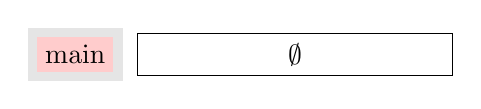
\begin{tikzpicture}[stack/.style={rectangle split, rectangle split parts=#1, draw, anchor=center, text centered},
        scope/.style={fill=gray!20, anchor=center}]
    \node[stack=1, minimum width=4.0cm] (s) {
    \nodepart{one} $\emptyset$
    };
    \node[scope, left=5pt of s.one west]   {\colorbox{red!20}{\scope{main}}};
    \end{tikzpicture}   
}
\end{minipage}
\end{figure}

\end{frame}


% ----

\begin{frame}[fragile]
\frametitle{The introductory example under the \cinkrestrict semantics}
\begin{minted}[escapeinside=||,mathescape=true,texcomments]{c}
// Scope \scope{foo}
int foo(int* restrict p, int* restrict q) {   
    *p = 10;
    *q = 11;
    return *p;
}
\end{minted}

\begin{figure}[h]
\centering
\begin{minipage}{.33\textwidth}
\begin{minted}[escapeinside=||,mathescape=true,texcomments]{c}
// Scope \scope{main}
int main() {
    |\colorbox{red!20}{int x;}| // $\&x = \Blockvar_x$
    foo(&x, &x);
}
\end{minted}
\end{minipage}%
\begin{minipage}{.67\textwidth}
\executionannotation
{
\{\colorbox{red!20}{$\Blockvar_x \mapsto \vundef$}\}
}
{
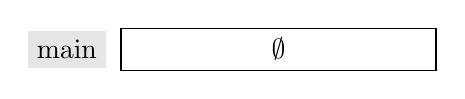
\begin{tikzpicture}[stack/.style={rectangle split, rectangle split parts=#1, draw, anchor=center, text centered},
        scope/.style={fill=gray!20, anchor=center}]
\node[stack=1, minimum width=4.0cm] (s) {
\nodepart{one} $\emptyset$
};
\node[scope, left=5pt of s.one west]   {\scope{main}};

\end{tikzpicture}
}
\end{minipage}
\end{figure}

\end{frame}


% ----

\begin{frame}[fragile]
\frametitle{The introductory example under the \cinkrestrict semantics}
\begin{minted}[escapeinside=||,mathescape=true,texcomments]{c}
// Scope \scope{foo} \quad $\&p = \Blockvar_p$ \quad $\&q = \Blockvar_q$
int foo(int* restrict p, int* restrict q) { 
    *p = 10;
    *q = 11;
    return *p;
}
\end{minted}

\begin{figure}[h]
\centering
\begin{minipage}{.33\textwidth}
\begin{minted}[escapeinside=||,mathescape=true,texcomments]{c}
// Scope \scope{main}
int main() {
    int x; // $\&x = \Blockvar_x$
    |\colorbox{red!20}{foo(&x, &x);}|
}
\end{minted}
\end{minipage}%
\begin{minipage}{.67\textwidth}
\executionannotation
{
\{\colorbox{red!20}{$\Blockvar_p \mapsto \ptr{(\Blockvar_x, \set{(\Blockvar_p, \scope{foo})})}$},\\
                                            \ \colorbox{red!20}{$\Blockvar_q \mapsto \ptr{(\Blockvar_x, \set{(\Blockvar_q, \scope{foo})})}$}, \\
                                            \ $\Blockvar_x \mapsto \vundef$\}
}
{
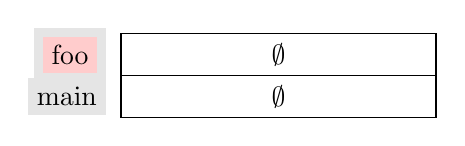
\begin{tikzpicture}[stack/.style={rectangle split, rectangle split parts=#1, draw, anchor=center, text centered},
        scope/.style={fill=gray!20, anchor=center}]
\node[stack=2, minimum width=4.0cm] (s) {
    \nodepart{one} $\emptyset$
    \nodepart{two} $\emptyset$
};
\node[scope, left=5pt of s.one west]   {\colorbox{red!20}{\scope{foo}}};
\node[scope, left=5pt of s.two west]   {\scope{main}};

\end{tikzpicture}
}
\end{minipage}
\end{figure}
\end{frame}

% ----

\begin{frame}[fragile]
\frametitle{The introductory example under the \cinkrestrict semantics}
\begin{minted}[escapeinside=||,mathescape=true,texcomments]{c}
// Scope \scope{foo} \quad $\&p = \Blockvar_p$ \quad $\&q = \Blockvar_q$
int foo(int* restrict p, int* restrict q) {   
    |\colorbox{red!20}{*p = 10;}|
    *q = 11;
    return *p;
}
\end{minted}

\begin{figure}[h]
\centering
\begin{minipage}{.33\textwidth}
\begin{minted}[escapeinside=||,mathescape=true,texcomments]{c}
// Scope \scope{main}
int main() {
    int x; // $\&x = \Blockvar_x$
    foo(&x, &x);
}
\end{minted}
\end{minipage}%
\begin{minipage}{.67\textwidth}
\executionannotation
{\{$\Blockvar_p \mapsto \ptr{(\Blockvar_x, \set{(\Blockvar_p, \scope{foo})})}$,\\
                                            \ $\Blockvar_q \mapsto \ptr{(\Blockvar_x, \set{(\Blockvar_q, \scope{foo})})}$, \\
                                            \ $\Blockvar_x \mapsto \colorbox{red!20}{10}$\}
}
{
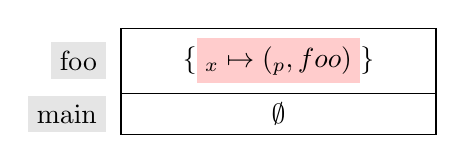
\begin{tikzpicture}[stack/.style={rectangle split, rectangle split parts=#1, draw, anchor=center, text centered},
        scope/.style={fill=gray!20, anchor=center}]
% Stack
\node[stack=2, minimum width=4.0cm] (s) {
    \nodepart{one} \{\colorbox{red!20}{$\Blockvar_x \mapsto \restricted{\set{(\Blockvar_p, \scope{foo})}}$}\}
    \nodepart{two} $\emptyset$
};

% Scopes
\node[scope, left=5pt of s.one west]   {\scope{foo}};
\node[scope, left=5pt of s.two west]   {\scope{main}};

\end{tikzpicture}
}
\end{minipage}
\end{figure}

\end{frame}


% ----

\begin{frame}[fragile]
\frametitle{The introductory example under the \cinkrestrict semantics}
\begin{minted}[escapeinside=||,mathescape=true,texcomments]{c}
// Scope \scope{foo} \quad $\&p = \Blockvar_p$ \quad $\&q = \Blockvar_q$
int foo(int* restrict p, int* restrict q) {   
    *p = 10;
    |\colorbox{red!20}{*q = 11;}|
    return *p;
}
\end{minted}
\vspace*{-30pt}
\begin{figure}[h]
\centering
\begin{minipage}{.33\textwidth}
\begin{minted}[escapeinside=||,mathescape=true,texcomments]{c}
// Scope \scope{main}
int main() {
    int x; // $\&x = \Blockvar_x$
    foo(&x, &x);
}
\end{minted}
\end{minipage}%
\begin{minipage}{.67\textwidth}
\colorbox{red!20}{$\restricted{\set{(\Blockvar_\text{\textcolor{blue}{$q$}}, \scope{foo})}} \joinsym \restricted{\set{(\Blockvar_\text{\textcolor{blue}{$p$}}, \scope{foo})}} = ...$}
\\

\executionannotation
{\{$\Blockvar_p \mapsto \ptr{(\Blockvar_x, \set{(\Blockvar_p, \scope{foo})})}$,\\
                                            \ $\Blockvar_q \mapsto \ptr{(\Blockvar_x, \set{(\Blockvar_q, \scope{foo})})}$, \\
                                            \ $\Blockvar_x \mapsto \vundef$\}
}
{
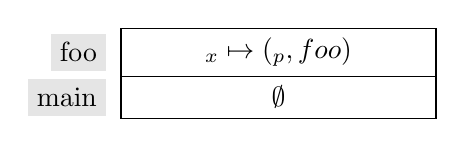
\begin{tikzpicture}[stack/.style={rectangle split, rectangle split parts=#1, draw, anchor=center, text centered},
        scope/.style={fill=gray!20, anchor=center}]
% Stack
\node[stack=2, minimum width=4.0cm] (s) {
    \nodepart{one} $\set{\Blockvar_x \mapsto \restricted{\set{(\Blockvar_p, \scope{foo})}}}$
    \nodepart{two} $\emptyset$
};

% Scopes
\node[scope, left=5pt of s.one west]   {\scope{foo}};
\node[scope, left=5pt of s.two west]   {\scope{main}};

\end{tikzpicture}
}
\end{minipage}
\end{figure}

\end{frame}




% ----

\begin{frame}[fragile]
\frametitle{The introductory example under the \cinkrestrict semantics}
\colorbox{red!20}{$\restricted{\set{(\Blockvar_\text{\textcolor{blue}{$q$}}, \scope{foo})}} \joinsym \restricted{\set{(\Blockvar_\text{\textcolor{blue}{$p$}}, \scope{foo})}} = ...$}

\begin{minipage}{.5\textwidth}
\begin{itemize}
    \item The symmetric \joinsym \ operation describes the result of joining two restrict states \\~\\
    \item \footnotesize$\unresabbr = \unrestricted$, $\resabbr{\Basesvar} = (\restricted{\Basesvar})$ and $\orabbr{\Basesvar} = (\onlyread{\Basesvar})$
    \item \footnotesize$\Basesvar \neq \Basesvar'$
\end{itemize}
\end{minipage}%
\begin{minipage}{.5\textwidth}

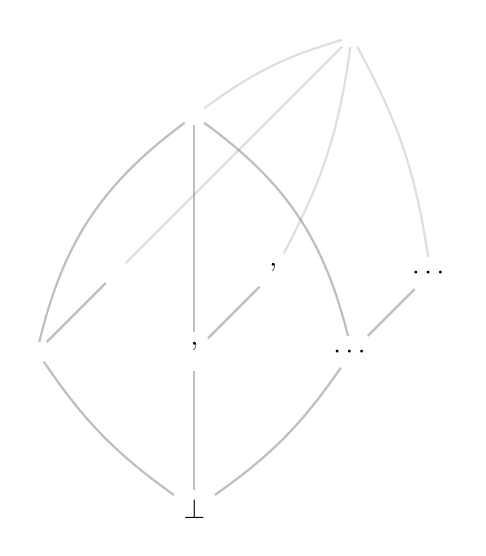
\begin{tikzpicture}
    \node (ub)     at (7,5) {\rsub};
    \node (un)     at (5,4) {\unresabbr};
    \node (rsbs)   at (4,2) {\resabbr{\Basesvar}};
    \node (rsbs')  at (6,2) {\resabbr{\Basesvar'}};
    \node (rsbs'') at (8,2) {$\cdots$};
    \node (orbs)   at (3,1) {\orabbr{\Basesvar}};
    \node (orbs')  at (5,1) {\orabbr{\Basesvar'}};
    \node (orbs'') at (7,1) {$\cdots$};
    \node (bot)    at (5,-1) {$\bot$};

    \path[thick, black, opacity=0.25]
    (bot) edge[bend left=10] node {} (orbs)
    (bot) edge node {} (orbs')
    (bot) edge[bend right=10] node {} (orbs'')
    
    (orbs) edge node {} (rsbs) 
    (orbs') edge node {} (rsbs')
    (orbs'') edge node {} (rsbs'')  
    
    (orbs) edge[bend left=20] node {} (un)
    (orbs') edge node {} (un)
    (orbs'') edge[bend right=20] node {} (un)

    (rsbs) edge[gray] node {} (ub)
    (rsbs') edge[bend right=10, gray] node {} (ub)
    (rsbs'') edge[bend right=10, gray] node {} (ub)

    (un) edge[bend left=10, gray] node {} (ub);
\end{tikzpicture}
\end{minipage}

\end{frame}


% ----

\begin{frame}[fragile]
\frametitle{The introductory example under the \cinkrestrict semantics}

\colorbox{red!20}{$\restricted{\set{(\Blockvar_\text{\textcolor{blue}{$q$}}, \scope{foo})}} \joinsym \restricted{\set{(\Blockvar_\text{\textcolor{blue}{$p$}}, \scope{foo})}} = \rsub$}

\begin{minipage}{.5\textwidth}
\begin{itemize}
    \item The symmetric \joinsym \ operation describes the result of joining two restrict states \\~\\
    \item \footnotesize$\unresabbr = \unrestricted$, $\resabbr{\Basesvar} = (\restricted{\Basesvar})$ and $\orabbr{\Basesvar} = (\onlyread{\Basesvar})$
    \item \footnotesize$\Basesvar \neq \Basesvar'$
\end{itemize}
\end{minipage}%
\begin{minipage}{.5\textwidth}

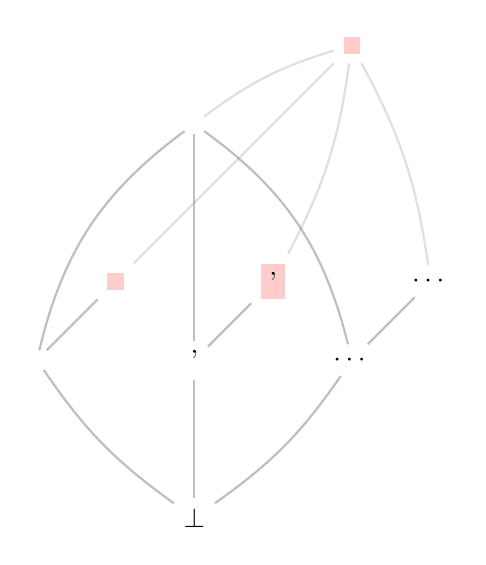
\begin{tikzpicture}
    \node (ub)     at (7,5) {\colorbox{red!20}{\rsub}};
    \node (un)     at (5,4) {\unresabbr};
    \node (rsbs)   at (4,2) {\colorbox{red!20}{\resabbr{\Basesvar}}};
    \node (rsbs')  at (6,2) {\colorbox{red!20}{\resabbr{\Basesvar'}}};
    \node (rsbs'') at (8,2) {$\cdots$};
    \node (orbs)   at (3,1) {\orabbr{\Basesvar}};
    \node (orbs')  at (5,1) {\orabbr{\Basesvar'}};
    \node (orbs'') at (7,1) {$\cdots$};
    \node (bot)    at (5,-1) {$\bot$};

    \path[thick, black, opacity=0.25]
    (bot) edge[bend left=10] node {} (orbs)
    (bot) edge node {} (orbs')
    (bot) edge[bend right=10] node {} (orbs'')
    
    (orbs) edge node {} (rsbs) 
    (orbs') edge node {} (rsbs')
    (orbs'') edge node {} (rsbs'')  
    
    (orbs) edge[bend left=20] node {} (un)
    (orbs') edge node {} (un)
    (orbs'') edge[bend right=20] node {} (un)

    (rsbs) edge[gray] node {} (ub)
    (rsbs') edge[bend right=10, gray] node {} (ub)
    (rsbs'') edge[bend right=10, gray] node {} (ub)

    (un) edge[bend left=10, gray] node {} (ub);
\end{tikzpicture}
\end{minipage}

\end{frame}

% ----

\begin{frame}[fragile]
\frametitle{The introductory example under the \cinkrestrict semantics}
\begin{minted}[escapeinside=||,mathescape=true,texcomments]{c}
// Scope \scope{foo} \quad $\&p = \Blockvar_p$ \quad $\&q = \Blockvar_q$
int foo(int* restrict p, int* restrict q) {   
    *p = 10;
    |\colorbox{red!20}{*q = 11;}|
    return *p;
}
\end{minted}
\vspace*{-30pt}
\begin{figure}[h]
\centering
\begin{minipage}{.33\textwidth}
\begin{minted}[escapeinside=||,mathescape=true,texcomments]{c}
// Scope \scope{main}
int main() {
    int x; // $\&x = \Blockvar_x$
    foo(&x, &x);
}
\end{minted}
\end{minipage}%
\begin{minipage}{.67\textwidth}
\textbf{UB}: \colorbox{red!20}{$\restricted{\set{(\Blockvar_\text{\textcolor{blue}{$q$}}, \scope{foo})}} \joinsym \restricted{\set{(\Blockvar_\text{\textcolor{blue}{$p$}}, \scope{foo})}} = \rsub$}
\\

\executionannotation
{\{$\Blockvar_p \mapsto \ptr{(\Blockvar_x, \set{(\Blockvar_p, \scope{foo})})}$,\\
                                            \ $\Blockvar_q \mapsto \ptr{(\Blockvar_x, \set{(\Blockvar_q, \scope{foo})})}$, \\
                                            \ $\Blockvar_x \mapsto \vundef$\}
}
{
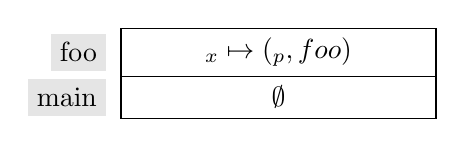
\begin{tikzpicture}[stack/.style={rectangle split, rectangle split parts=#1, draw, anchor=center, text centered},
        scope/.style={fill=gray!20, anchor=center}]
% Stack
\node[stack=2, minimum width=4.0cm] (s) {
    \nodepart{one} $\set{\Blockvar_x \mapsto \restricted{\set{(\Blockvar_p, \scope{foo})}}}$
    \nodepart{two} $\emptyset$
};

% Scopes
\node[scope, left=5pt of s.one west]   {\scope{foo}};
\node[scope, left=5pt of s.two west]   {\scope{main}};

\end{tikzpicture}
}
\end{minipage}
\end{figure}

\end{frame}



\begin{frame}
\frametitle{Evaluating the \cinkrestrict semantics}
\begin{itemize}
\item The semantics correctly gives undefined behavior to our introductory example! \\ \ But, we argue, there are some problems: \\
\item Too much undefined behavior (TMU)
    \begin{itemize}
        \item \colorbox{ao!20}{Aliasing loads}
        \item Returning restrict pointers
    \end{itemize}
\item Too little undefined behavior (TLU)
    \begin{itemize}
        \item Array of restrict pointers
        \item Nested restrict pointers
        \item Semantic preservation under inlining
        \item Call to free  
    \end{itemize}
\end{itemize}

\end{frame}

\begin{frame}[fragile]
\frametitle{Aliasing loads (TMU)}
\begin{minipage}{0.7\textwidth}
\begin{minted}[escapeinside=||,mathescape=true,linenos]{c}
// Scope $\scope{h}$
void h(int* q, int* restrict r, int* restrict s) {
    *q = *r + *s; 
}
// Scope $\scope{main}$
int main() {
    int x, y;
    int* restrict p = &y;
    *p = 0; 
    h(&x, p, p);
}
\end{minted}
\end{minipage}%
\begin{minipage}[t]{0.3\textwidth}
\begin{tikzpicture}
    \node (q) {\mintinline{c}{q}};
    \node[right of = q] (pointee-q) {$x$};

    \node[right of = pointee-p] (rs) {\mintinline{c}{r,s}};
    \node[right of = rs] (pointee-rs) {$y$};

    \draw[->] (q) -- (pointee-q);
    \draw[->] (rs) -- (pointee-rs);
\end{tikzpicture}
\end{minipage}

\begin{itemize}
    \item Simplified version of example 3 from the ISO standard demonstrating DB
    \item $y$ does \textbf{not} get \textbf{modified} in the scope \scope{h} of \mintinline{c}{r,s}
\end{itemize}

\end{frame}


% ----


\begin{frame}[fragile]
\frametitle{Aliasing loads (TMU)}
\begin{minted}[escapeinside=||,mathescape=true]{c}
// Scope $\scope{h}$
void h(int* q, int* restrict r, int* restrict s) {
    *q = *r + *s; 
}
\end{minted}

\begin{figure}[h]
\centering
\begin{minipage}{.36\textwidth}
\begin{minted}[escapeinside=||,mathescape=true]{c}
// Scope $\scope{main}$
|\colorbox{red!20}{int main() \{}|
    int x, y;
    int* restrict p = &y;
    *p = 0; 
    h(&x, p, p);
}
\end{minted}
\end{minipage}%
\begin{minipage}{.674\textwidth}
\executionannotation
{
    $\emptyset$
}
{
    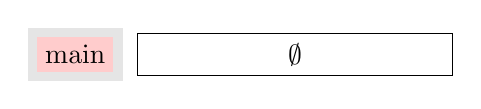
\begin{tikzpicture}[stack/.style={rectangle split, rectangle split parts=#1, draw, anchor=center, text centered},
        scope/.style={fill=gray!20, anchor=center}]
    \node[stack=1, minimum width=4.0cm] (s) {
    \nodepart{one} $\emptyset$
    };
    \node[scope, left=5pt of s.one west]   {\colorbox{red!20}{\scope{main}}};
    \end{tikzpicture}   
}
\end{minipage}
\end{figure}

\end{frame}


% ----


\begin{frame}[fragile]
\frametitle{Aliasing loads (TMU)}
\begin{minted}[escapeinside=||,mathescape=true]{c}
// Scope $\scope{h}$
void h(int* q, int* restrict r, int* restrict s) {
    *q = *r + *s; 
}
\end{minted}

\begin{figure}[h]
\centering
\begin{minipage}{.36\textwidth}
\begin{minted}[escapeinside=||,mathescape=true]{c}
// Scope $\scope{main}$
int main() {
    |\colorbox{red!20}{int x, y;}|
    int* restrict p = &y;
    *p = 0; 
    h(&x, p, p);
}
\end{minted}
\end{minipage}%
\begin{minipage}{.64\textwidth}
\executionannotation
{
\{\colorbox{red!20}{$\Blockvar_x \mapsto \vundef, \Blockvar_y \mapsto \vundef$}\}
}
{
    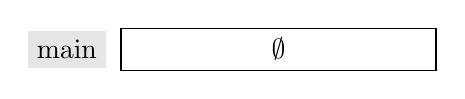
\begin{tikzpicture}[stack/.style={rectangle split, rectangle split parts=#1, draw, anchor=center, text centered},
        scope/.style={fill=gray!20, anchor=center}]
    \node[stack=1, minimum width=4.0cm] (s) {
    \nodepart{one} $\emptyset$
    };
    \node[scope, left=5pt of s.one west]   {\scope{main}};
    \end{tikzpicture}   
}
\end{minipage}
\end{figure}

\end{frame}


% ---- 


\begin{frame}[fragile]
\frametitle{Aliasing loads (TMU)}
\begin{minted}[escapeinside=||,mathescape=true]{c}
// Scope $\scope{h}$
void h(int* q, int* restrict r, int* restrict s) {
    *q = *r + *s; 
}
\end{minted}

\begin{figure}[h]
\centering
\begin{minipage}{.36\textwidth}
\begin{minted}[escapeinside=||,mathescape=true]{c}
// Scope $\scope{main}$
int main() {
    int x, y;
    |\colorbox{red!20}{int* restrict p = &y;}|
    *p = 0;
    h(&x, p, p);
}
\end{minted}
\end{minipage}%
\begin{minipage}{.64\textwidth}
\executionannotation
{
\{$\Blockvar_x \mapsto \vundef$, \\
    \ $\Blockvar_y \mapsto \vundef$, \\
    \ \colorbox{red!20}{$\Blockvar_p \mapsto \ptr{(\Blockvar_y, \set{(\Blockvar_p, \scope{main})})}$}
\}
}
{
    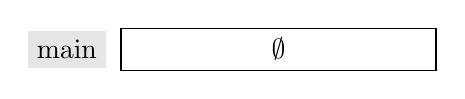
\begin{tikzpicture}[stack/.style={rectangle split, rectangle split parts=#1, draw, anchor=center, text centered},
        scope/.style={fill=gray!20, anchor=center}]
    \node[stack=1, minimum width=4.0cm] (s) {
    \nodepart{one} $\emptyset$
    };
    \node[scope, left=5pt of s.one west]   {\scope{main}};
    \end{tikzpicture}   
}
\end{minipage}
\end{figure}


\end{frame}


% ---- 


\begin{frame}[fragile]
\frametitle{Aliasing loads (TMU)}
\begin{minted}[escapeinside=||,mathescape=true]{c}
// Scope $\scope{h}$
void h(int* q, int* restrict r, int* restrict s) {
    *q = *r + *s; 
}
\end{minted}

\begin{figure}[h]
\centering
\begin{minipage}{.36\textwidth}
\begin{minted}[escapeinside=||,mathescape=true]{c}
// Scope $\scope{main}$
int main() {
    int x, y;
    int* restrict p = &y;
    |\colorbox{red!20}{*p = 0;}|
    h(&x, p, p);
}
\end{minted}
\end{minipage}%
\begin{minipage}{.64\textwidth}
\executionannotation
{
\{$\Blockvar_x \mapsto \vundef$, \\
    \ $\Blockvar_y \mapsto \colorbox{red!20}{0}$, \\
    \ $\Blockvar_p \mapsto \ptr{(\Blockvar_y, \set{(\Blockvar_p, \scope{main})})}$
\}
}
{
    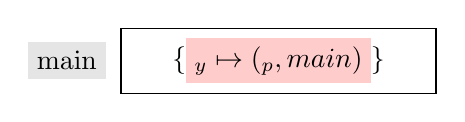
\begin{tikzpicture}[stack/.style={rectangle split, rectangle split parts=#1, draw, anchor=center, text centered},
        scope/.style={fill=gray!20, anchor=center}]
    \node[stack=1, minimum width=4.0cm] (s) {
    \nodepart{one} \{\colorbox{red!20}{$\Blockvar_y \mapsto \restricted{\set{(\Blockvar_p, \scope{main})}}$}\}
    };
    \node[scope, left=5pt of s.one west]   {\scope{main}};
    \end{tikzpicture}   
}
\end{minipage}
\end{figure}


\end{frame}


% ---- 


\begin{frame}[fragile]
\frametitle{Aliasing loads (TMU)}
\begin{minted}[escapeinside=||,mathescape=true]{c}
// Scope $\scope{h}$
void h(int* q, int* restrict r, int* restrict s) {
    *q = *r + *s; 
}
\end{minted}
\vspace*{-1cm}
\begin{figure}[h]
\centering
\begin{minipage}{.36\textwidth}
\begin{minted}[escapeinside=||,mathescape=true]{c}
// Scope $\scope{main}$
int main() {
    int x, y;
    int* restrict p = &y;
    *p = 0;
    |\colorbox{red!20}{h(&x, p, p);}|
}
\end{minted}
\end{minipage}%
\begin{minipage}{.64\textwidth}
\executionannotation
{
\{$\Blockvar_x \mapsto \vundef$, $\Blockvar_y \mapsto 0$, \\
    \ $\Blockvar_p \mapsto \ptr{(\Blockvar_y, \set{(\Blockvar_p, \scope{main})})}$, \\
    \ \colorbox{red!20}{$\Blockvar_q \mapsto \ptr{(\Blockvar_x, \emptyset)}$}, \\
    \ \colorbox{red!20}{$\Blockvar_r \mapsto \ptr{(\Blockvar_y, \set{(\Blockvar_r, \scope{h}), (\Blockvar_p, \scope{main})})} $}, \\
    \ \colorbox{red!20}{$\Blockvar_s \mapsto \ptr{(\Blockvar_y, \set{(\Blockvar_s, \scope{h}), (\Blockvar_p, \scope{main})})} $} \\
\}
}
{
    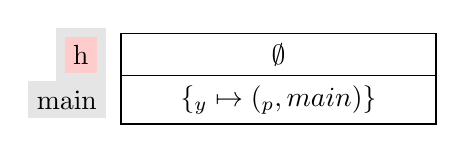
\begin{tikzpicture}[stack/.style={rectangle split, rectangle split parts=#1, draw, anchor=center, text centered},
        scope/.style={fill=gray!20, anchor=center}]
    \node[stack=2, minimum width=4.0cm] (s) {
    \nodepart{one} $\emptyset$
    \nodepart{two} \{$\Blockvar_y \mapsto \restricted{\set{(\Blockvar_p, \scope{main})}}$\}
    };
    \node[scope, left=5pt of s.one west]   {\colorbox{red!20}{\scope{h}}};
    \node[scope, left=5pt of s.two west]   {\scope{main}};
    \end{tikzpicture}   
}
\end{minipage}
\end{figure}

\end{frame}



% ---- 


\begin{frame}[fragile]
\frametitle{Aliasing loads (TMU)}
\begin{minted}[escapeinside=||,mathescape=true]{c}
// Scope $\scope{h}$
void h(int* q, int* restrict r, int* restrict s) {
    *q = |\colorbox{red!20}{*r}| + *s; 
}
\end{minted}
\vspace*{-1cm}
\begin{figure}[!h]
\begin{minipage}[t]{.36\textwidth}

\begin{minted}[escapeinside=||,mathescape=true]{c}
// Scope $\scope{main}$
int main() {
    int x, y;
    int* restrict p = &y;
    *p = 0;
    h(&x, p, p);
}
\end{minted}
\end{minipage}%
\begin{minipage}{.64\textwidth}
\executionannotation
{
\{$\Blockvar_x \mapsto \vundef$, $\Blockvar_y \mapsto 0$, \\
    \ $\Blockvar_p \mapsto \ptr{(\Blockvar_y, \set{(\Blockvar_p, \scope{main})})}$, \\
    \ $\Blockvar_q \mapsto \ptr{(\Blockvar_x, \emptyset)}$, \\
    \ $\Blockvar_r \mapsto \ptr{(\Blockvar_y, \set{(\Blockvar_r, \scope{h}), (\Blockvar_p, \scope{main})})} $, \\
    \ $\Blockvar_s \mapsto \ptr{(\Blockvar_y, \set{(\Blockvar_s, \scope{h}), (\Blockvar_p, \scope{main})})} $ \\
\}
}
{
    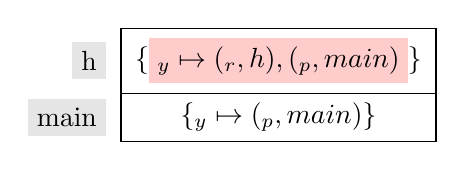
\begin{tikzpicture}[stack/.style={rectangle split, rectangle split parts=#1, draw, anchor=center, text centered},
        scope/.style={fill=gray!20, anchor=center}]
    \node[stack=2, minimum width=4.0cm] (s) {
    \nodepart{one} \{\colorbox{red!20}{$\Blockvar_y \mapsto \onlyread{\set{(\Blockvar_r, \scope{h}), (\Blockvar_p, \scope{main})}}$}\}
    \nodepart{two} \{$\Blockvar_y \mapsto \restricted{\set{(\Blockvar_p, \scope{main})}}$\}
    };
    \node[scope, left=5pt of s.one west]   {\scope{h}};
    \node[scope, left=5pt of s.two west]   {\scope{main}};
    \end{tikzpicture}   
}
\end{minipage}
\end{figure}

\end{frame}

% ---- 


\begin{frame}[fragile]
\frametitle{Aliasing loads (TMU)}
\begin{minted}[escapeinside=||,mathescape=true]{c}
// Scope $\scope{h}$
void h(int* q, int* restrict r, int* restrict s) {
    *q = *r + |\colorbox{red!20}{*s}|; 
}
\end{minted}
\vspace*{-1cm}
\begin{figure}[!h]
\begin{minipage}[t]{.36\textwidth}

\begin{minted}[escapeinside=||,mathescape=true]{c}
// Scope $\scope{main}$
int main() {
    int x, y;
    int* restrict p = &y;
    *p = 0;
    h(&x, p, p);
}
\end{minted}
\end{minipage}%
\begin{minipage}{.64\textwidth}
\colorbox{red!20}{$\onlyread{\set{(\Blockvar_\text{\textcolor{blue}{$r$}}, \scope{h}), (\Blockvar_p, \scope{main})}} \joinsym $} \\
\colorbox{red!20}{$\onlyread{\set{(\Blockvar_\text{\textcolor{blue}{$s$}}, \scope{h}), (\Blockvar_p, \scope{main})}} = ...$}
\\

\executionannotation
{
\{..., \\\  $\Blockvar_r \mapsto \ptr{(\Blockvar_y, \set{(\Blockvar_r, \scope{h}), (\Blockvar_p, \scope{main})})} $, \\
         \ $\Blockvar_s \mapsto \ptr{(\Blockvar_y, \set{(\Blockvar_s, \scope{h}), (\Blockvar_p, \scope{main})})}$ \}
}
{
    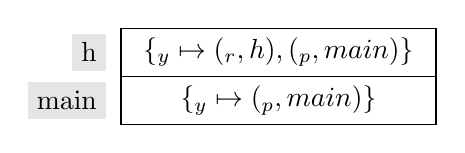
\begin{tikzpicture}[stack/.style={rectangle split, rectangle split parts=#1, draw, anchor=center, text centered},
        scope/.style={fill=gray!20, anchor=center}]
    \node[stack=2, minimum width=4.0cm] (s) {
    \nodepart{one} \{$\Blockvar_y \mapsto \onlyread{\set{(\Blockvar_r, \scope{h}), (\Blockvar_p, \scope{main})}}$\}
    \nodepart{two} \{$\Blockvar_y \mapsto \restricted{\set{(\Blockvar_p, \scope{main})}}$\}
    };
    \node[scope, left=5pt of s.one west]   {\scope{h}};
    \node[scope, left=5pt of s.two west]   {\scope{main}};
    \end{tikzpicture}   
}
\end{minipage}
\end{figure}

\end{frame}


% ----


\begin{frame}[fragile]
\frametitle{Aliasing loads (TMU)}
\centering
\colorbox{red!20}{$\onlyread{\set{(\Blockvar_\text{\textcolor{blue}{$r$}}, \scope{h}), (\Blockvar_p, \scope{main})}} \joinsym \ \onlyread{\set{(\Blockvar_\text{\textcolor{blue}{$s$}}, \scope{h}), (\Blockvar_p, \scope{main})}} = \unrestricted$}

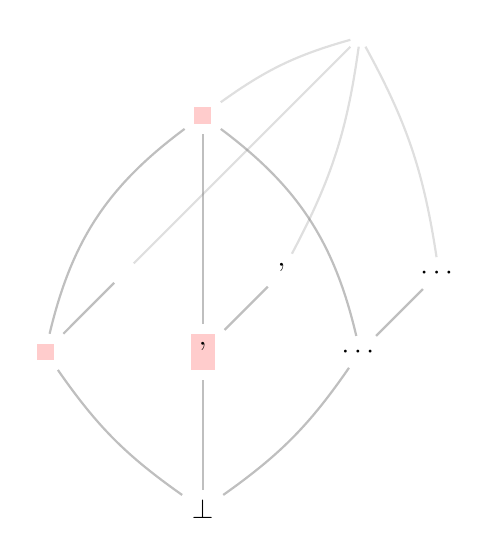
\begin{tikzpicture}
    \node (ub)     at (7,5) {\rsub};
    \node (un)     at (5,4) {\colorbox{red!20}{\unresabbr}};
    \node (rsbs)   at (4,2) {\resabbr{\Basesvar}};
    \node (rsbs')  at (6,2) {\resabbr{\Basesvar'}};
    \node (rsbs'') at (8,2) {$\cdots$};
    \node (orbs)   at (3,1) {\colorbox{red!20}{\orabbr{\Basesvar}}};
    \node (orbs')  at (5,1) {\colorbox{red!20}{\orabbr{\Basesvar'}}};
    \node (orbs'') at (7,1) {$\cdots$};
    \node (bot)    at (5,-1) {$\bot$};

    \path[thick, black, opacity=0.25]
    (bot) edge[bend left=10] node {} (orbs)
    (bot) edge node {} (orbs')
    (bot) edge[bend right=10] node {} (orbs'')
    
    (orbs) edge node {} (rsbs) 
    (orbs') edge node {} (rsbs')
    (orbs'') edge node {} (rsbs'')  
    
    (orbs) edge[bend left=20] node {} (un)
    (orbs') edge node {} (un)
    (orbs'') edge[bend right=20] node {} (un)

    (rsbs) edge[gray] node {} (ub)
    (rsbs') edge[bend right=10, gray] node {} (ub)
    (rsbs'') edge[bend right=10, gray] node {} (ub)

    (un) edge[bend left=10, gray] node {} (ub);
\end{tikzpicture}

\end{frame}

    
% ---- 


\begin{frame}[fragile]
\frametitle{Aliasing loads (TMU)}
\begin{minted}[escapeinside=||,mathescape=true]{c}
// Scope $\scope{h}$
void h(int* q, int* restrict r, int* restrict s) {
    *q = *r + |\colorbox{red!20}{*s}|; 
}
\end{minted}

\vspace*{-1cm}

\begin{figure}[!h]
\begin{minipage}[t]{.36\textwidth}

\begin{minted}[escapeinside=||,mathescape=true]{c}
// Scope $\scope{main}$
int main() {
    int x, y;
    int* restrict p = &y;
    *p = 0;
    h(&x, p, p);
}
\end{minted}
\end{minipage}%
\begin{minipage}{.64\textwidth}

\executionannotation
{
\{..., \\\  $\Blockvar_r \mapsto \ptr{(\Blockvar_y, \set{(\Blockvar_r, \scope{h}), (\Blockvar_p, \scope{main})})} $, \\
            \ $\Blockvar_s \mapsto \ptr{(\Blockvar_y, \set{(\Blockvar_s, \scope{h}), (\Blockvar_p, \scope{main})})}$ \}
}
{
    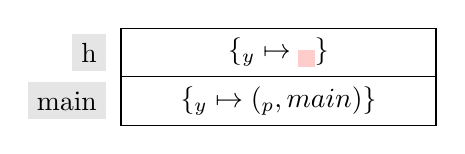
\begin{tikzpicture}[stack/.style={rectangle split, rectangle split parts=#1, draw, anchor=center, text centered},
        scope/.style={fill=gray!20, anchor=center}]
    \node[stack=2, minimum width=4.0cm] (s) {
    \nodepart{one} \{$\Blockvar_y \mapsto \colorbox{red!20}{\unrestricted}$\}
    \nodepart{two} \{$\Blockvar_y \mapsto \restricted{\set{(\Blockvar_p, \scope{main})}}$\}
    };
    \node[scope, left=5pt of s.one west]   {\scope{h}};
    \node[scope, left=5pt of s.two west]   {\scope{main}};
    \end{tikzpicture}   
}
\end{minipage}
\end{figure}

\end{frame}


% ---- 


\begin{frame}[fragile]
\frametitle{Aliasing loads (TMU)}
\begin{minted}[escapeinside=||,mathescape=true]{c}
// Scope $\scope{h}$
void h(int* q, int* restrict r, int* restrict s) {
    *q = *r + *s; 
|\colorbox{red!20}{\}}|
\end{minted}

\vspace*{-1cm}

\begin{figure}[!h]
\begin{minipage}[t]{.36\textwidth}

\begin{minted}[escapeinside=||,mathescape=true]{c}
// Scope $\scope{main}$
int main() {
    int x, y;
    int* restrict p = &y;
    *p = 0;
    h(&x, p, p);
}
\end{minted}
\end{minipage}%
\begin{minipage}{.64\textwidth}

\executionannotation
{
\{..., \\\  $\Blockvar_r \mapsto \ptr{(\Blockvar_y, \set{(\Blockvar_r, \scope{h}), (\Blockvar_p, \scope{main})})} $, \\
            \ $\Blockvar_s \mapsto \ptr{(\Blockvar_y, \set{(\Blockvar_s, \scope{h}), (\Blockvar_p, \scope{main})})}$ \}
}
{
    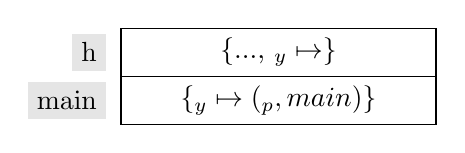
\begin{tikzpicture}[stack/.style={rectangle split, rectangle split parts=#1, draw, anchor=center, text centered},
        scope/.style={fill=gray!20, anchor=center}]
    \node[stack=2, minimum width=4.0cm] (s) {
    \nodepart{one} \{..., $\Blockvar_y \mapsto \unrestricted$\}
    \nodepart{two} \{$\Blockvar_y \mapsto \restricted{\set{(\Blockvar_p, \scope{main})}}$\}
    };
    \node[scope, left=5pt of s.one west]   {\scope{h}};
    \node[scope, left=5pt of s.two west]   {\scope{main}};
    \end{tikzpicture}   
}
\end{minipage}
\end{figure}

\end{frame}

    
% ---- 


\begin{frame}[fragile]
\frametitle{Aliasing loads (TMU)}

\begin{itemize}
    \item \scope{h} is part of the execution of scope \scope{main}
    \item Join the restrict states when \scope{h} terminates!
\end{itemize}
\leavevmode\\
\begin{tikzpicture}[stack/.style={rectangle split, rectangle split parts=#1, draw, anchor=center, text centered},
    scope/.style={fill=gray!20, anchor=center}]
\node[stack=2, minimum width=4.0cm] (s) {
\nodepart{one} \{$\Blockvar_y \mapsto \unrestricted$\}
\nodepart{two} \{$\Blockvar_y \mapsto \restricted{\set{(\Blockvar_p, \scope{main})}}$\}
};
\node[scope, left=5pt of s.one west]   {\scope{h}};
\node[scope, left=5pt of s.two west]   {\scope{main}};

\draw[->, dashed, thick] (s.one east) to[bend left=90, looseness=3] node[right] {$\joinsym$} (s.two east);

\end{tikzpicture}

\end{frame}


\begin{frame}[fragile]
\frametitle{Aliasing loads (TMU)}
\centering
\colorbox{red!20}{$\restricted{\set{(\Blockvar_p, \scope{main})}} \joinsym \unrestricted = \rsub$}

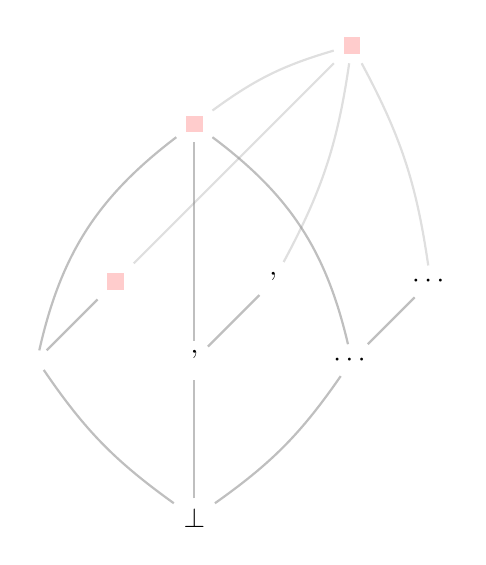
\begin{tikzpicture}
    \node (ub)     at (7,5) {\colorbox{red!20}{\rsub}};
    \node (un)     at (5,4) {\colorbox{red!20}{\unresabbr}};
    \node (rsbs)   at (4,2) {\colorbox{red!20}{\resabbr{\Basesvar}}};
    \node (rsbs')  at (6,2) {\resabbr{\Basesvar'}};
    \node (rsbs'') at (8,2) {$\cdots$};
    \node (orbs)   at (3,1) {\orabbr{\Basesvar}};
    \node (orbs')  at (5,1) {\orabbr{\Basesvar'}};
    \node (orbs'') at (7,1) {$\cdots$};
    \node (bot)    at (5,-1) {$\bot$};

    \path[thick, black, opacity=0.25]
    (bot) edge[bend left=10] node {} (orbs)
    (bot) edge node {} (orbs')
    (bot) edge[bend right=10] node {} (orbs'')
    
    (orbs) edge node {} (rsbs) 
    (orbs') edge node {} (rsbs')
    (orbs'') edge node {} (rsbs'')  
    
    (orbs) edge[bend left=20] node {} (un)
    (orbs') edge node {} (un)
    (orbs'') edge[bend right=20] node {} (un)

    (rsbs) edge[gray] node {} (ub)
    (rsbs') edge[bend right=10, gray] node {} (ub)
    (rsbs'') edge[bend right=10, gray] node {} (ub)

    (un) edge[bend left=10, gray] node {} (ub);
\end{tikzpicture}

\end{frame}


% ----


\begin{frame}[fragile]
\frametitle{Aliasing loads (TMU)}
\begin{itemize}
    \item The fundamental problem with $\unrestricted$ is \textbf{information loss}
    \item Idea: \textbf{remove} $\unrestricted$ entirely and promote $(\onlyread{\Basesvar})$ to $(\onlyread{\textdom{fbas}})$ with $\textdom{fbas} \in \Set{\Bases}$, \ie
    a \textbf{family of sets of bases}
    \begin{itemize}
        \item Every set of the family represents a pointer used for a load \\
        \item if $|\Basesfamvar| > 1$              \qquad the semantics of $\unrestricted$ apply
        \item if $\Basesfamvar = \set{\Basesvar}$ \;   the semantics of $(\onlyread{\Basesvar})$ apply
    \end{itemize}
\end{itemize}
\end{frame}

% ---- 


\begin{frame}[fragile]
\frametitle{Aliasing loads (TMU)}
\begin{minted}[escapeinside=||,mathescape=true]{c}
// Scope $\scope{h}$
void h(int* q, int* restrict r, int* restrict s) {
    *q = *r + |\colorbox{red!20}{*s}|; 
}
\end{minted}
\vspace*{-1cm}
\begin{figure}[!h]
\begin{minipage}[t]{.36\textwidth}

\begin{minted}[escapeinside=||,mathescape=true]{c}
// Scope $\scope{main}$
int main() {
    int x, y;
    int* restrict p = &y;
    *p = 0;
    h(&x, p, p);
}
\end{minted}
\end{minipage}%
\begin{minipage}{.64\textwidth}
\colorbox{red!20}{$\onlyread{\set{\set{(\Blockvar_\text{\textcolor{blue}{$r$}}, \scope{h}), (\Blockvar_p, \scope{main})}}} \joinsym $} \\
\colorbox{red!20}{$\onlyread{\set{\set{(\Blockvar_\text{\textcolor{blue}{$s$}}, \scope{h}), (\Blockvar_p, \scope{main})}}} = ...$}
\\

\executionannotation
{
\{..., \\\  $\Blockvar_r \mapsto \ptr{(\Blockvar_y, \set{(\Blockvar_r, \scope{h}), (\Blockvar_p, \scope{main})})} $, \\
            \ $\Blockvar_s \mapsto \ptr{(\Blockvar_y, \set{(\Blockvar_s, \scope{h}), (\Blockvar_p, \scope{main})})}$ \}
}
{
    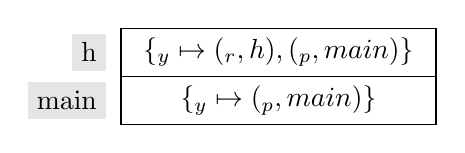
\begin{tikzpicture}[stack/.style={rectangle split, rectangle split parts=#1, draw, anchor=center, text centered},
        scope/.style={fill=gray!20, anchor=center}]
    \node[stack=2, minimum width=4.0cm] (s) {
    \nodepart{one} \{$\Blockvar_y \mapsto \onlyread{\set{\set{(\Blockvar_r, \scope{h}), (\Blockvar_p, \scope{main})}}}$\}
    \nodepart{two} \{$\Blockvar_y \mapsto \restricted{\set{(\Blockvar_p, \scope{main})}}$\}
    };
    \node[scope, left=5pt of s.one west]   {\scope{h}};
    \node[scope, left=5pt of s.two west]   {\scope{main}};
    \end{tikzpicture}   
}
\end{minipage}
\end{figure}

\end{frame}


% ---- 


\begin{frame}[fragile]
\frametitle{Aliasing loads (TMU)}
\centering
\colorbox{red!20}{$\onlyread{\set{\set{(\Blockvar_\text{\textcolor{blue}{$r$}}, \scope{h}), (\Blockvar_p, \scope{main})}}} \joinsym \onlyread{\set{\set{(\Blockvar_\text{\textcolor{blue}{$s$}}, \scope{h}), (\Blockvar_p, \scope{main})}}} = ...$}
\\

\begin{minipage}{.43\textwidth}
\begin{itemize}
    \item The updated symmetric \joinsym \ operation (simplified)
    \item $\Basesvar \neq \Basesvar'$
\end{itemize}
\end{minipage}%
\begin{minipage}{.57\textwidth}
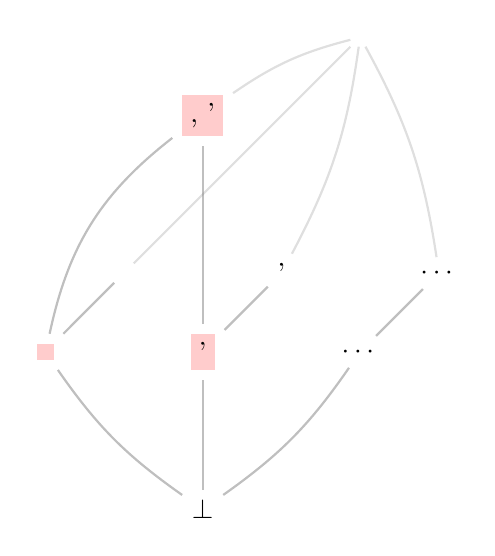
\begin{tikzpicture}
    \node (ub)     at (7,5) {\rsub};
    \node (un)     at (5,4) {\colorbox{red!20}{\orabbr{\set{\Basesvar, \Basesvar'}}}};
    \node (rsbs)   at (4,2) {\resabbr{\Basesvar}};
    \node (rsbs')  at (6,2) {\resabbr{\Basesvar'}};
    \node (rsbs'') at (8,2) {$\cdots$};
    \node (orbs)   at (3,1) {\colorbox{red!20}{\orabbr{\set{\Basesvar}}}};
    \node (orbs')  at (5,1) {\colorbox{red!20}{\orabbr{\set{\Basesvar'}}}};
    \node (orbs'') at (7,1) {$\cdots$};
    \node (bot)    at (5,-1) {$\bot$};

    \path[thick, black, opacity=0.25]
    (bot) edge[bend left=10] node {} (orbs)
    (bot) edge node {} (orbs')
    (bot) edge[bend right=10] node {} (orbs'')
    
    (orbs) edge node {} (rsbs) 
    (orbs') edge node {} (rsbs')
    (orbs'') edge node {} (rsbs'')  
    
    (orbs) edge[bend left=20] node {} (un)
    (orbs') edge node {} (un)
    % (orbs'') edge[bend right=20] node {} (un)

    (rsbs) edge[gray] node {} (ub)
    (rsbs') edge[bend right=10, gray] node {} (ub)
    (rsbs'') edge[bend right=10, gray] node {} (ub)

    (un) edge[bend left=10, gray] node {} (ub);
\end{tikzpicture}
\end{minipage}

\end{frame}




% ---- 


\begin{frame}[fragile]
\frametitle{Aliasing loads (TMU)}
\begin{minted}[escapeinside=||,mathescape=true]{c}
// Scope $\scope{h}$
void h(int* q, int* restrict r, int* restrict s) {
    *q = *r + |\colorbox{red!20}{*s}|; 
}
\end{minted}
\vspace*{-1cm}
\begin{figure}[!h]
\begin{minipage}[t]{.36\textwidth}

\begin{minted}[escapeinside=||,mathescape=true]{c}
// Scope $\scope{main}$
int main() {
    int x, y;
    int* restrict p = &y;
    *p = 0;
    h(&x, p, p);
}
\end{minted}
\end{minipage}%
\begin{minipage}{.64\textwidth}

\executionannotation
{
\{..., \\\  $\Blockvar_r \mapsto \ptr{(\Blockvar_y, \set{(\Blockvar_r, \scope{h}), (\Blockvar_p, \scope{main})})} $, \\
            \ $\Blockvar_s \mapsto \ptr{(\Blockvar_y, \set{(\Blockvar_s, \scope{h}), (\Blockvar_p, \scope{main})})}$ \}
}
{
    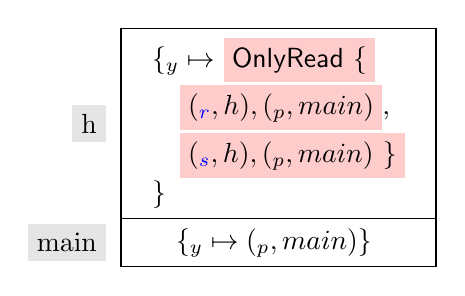
\begin{tikzpicture}[stack/.style={rectangle split, rectangle split parts=#1, draw, anchor=center, text centered,align=left},
        scope/.style={fill=gray!20, anchor=center}]
    \node[stack=2, minimum width=4.0cm] (s) {
    \nodepart[align=left]{one} \{$\Blockvar_y \mapsto$ \colorbox{red!20}{$\mathsf{OnlyRead}$ \{} \\
                                \quad \colorbox{red!20}{$\set{(\Blockvar_\text{\textcolor{blue}{$r$}}, \scope{h}), (\Blockvar_p, \scope{main})}$}, \\
                                \quad \colorbox{red!20}{$\set{(\Blockvar_\text{\textcolor{blue}{$s$}}, \scope{h}), (\Blockvar_p, \scope{main})}$ \}} \\ \}
                    
                   
    \nodepart{two} \{$\Blockvar_y \mapsto \restricted{\set{(\Blockvar_p, \scope{main})}}$\}
    };
    \node[scope, left=5pt of s.one west]   {\scope{h}};
    \node[scope, left=5pt of s.two west]   {\scope{main}};
    \end{tikzpicture}   
}
\end{minipage}
\end{figure}

\end{frame}


% ---- 


\begin{frame}[fragile]
\frametitle{Aliasing loads (TMU)}
\begin{minted}[escapeinside=||,mathescape=true]{c}
// Scope $\scope{h}$
void h(int* q, int* restrict r, int* restrict s) {
    *q = *r + *s; 
|\colorbox{red!20}{\}}|
\end{minted}
\vspace*{-1cm}
\begin{figure}[!h]
\begin{minipage}[t]{.36\textwidth}

\begin{minted}[escapeinside=||,mathescape=true]{c}
// Scope $\scope{main}$
int main() {
    int x, y;
    int* restrict p = &y;
    *p = 0;
    h(&x, p, p);
}
\end{minted}
\end{minipage}%
\begin{minipage}{.64\textwidth}

\executionannotation
{
\{..., \\\  $\Blockvar_r \mapsto \ptr{(\Blockvar_y, \set{(\Blockvar_r, \scope{h}), (\Blockvar_p, \scope{main})})} $, \\
            \ $\Blockvar_s \mapsto \ptr{(\Blockvar_y, \set{(\Blockvar_s, \scope{h}), (\Blockvar_p, \scope{main})})}$ \}
}
{
    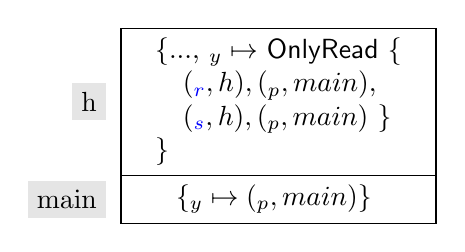
\begin{tikzpicture}[stack/.style={rectangle split, rectangle split parts=#1, draw, anchor=center, text centered,align=left},
        scope/.style={fill=gray!20, anchor=center}]
    \node[stack=2, minimum width=4.0cm] (s) {
    \nodepart[align=left]{one} \{...,  $\Blockvar_y \mapsto$ $\mathsf{OnlyRead}$ \{ \\
                                \quad $\set{(\Blockvar_\text{\textcolor{blue}{$r$}}, \scope{h}), (\Blockvar_p, \scope{main})}$, \\
                                \quad $\set{(\Blockvar_\text{\textcolor{blue}{$s$}}, \scope{h}), (\Blockvar_p, \scope{main})}$ \} \\ \}
                    
                    
    \nodepart{two} \{$\Blockvar_y \mapsto \restricted{\set{(\Blockvar_p, \scope{main})}}$\}
    };
    \node[scope, left=5pt of s.one west]   {\scope{h}};
    \node[scope, left=5pt of s.two west]   {\scope{main}};
    \end{tikzpicture}   
}
\end{minipage}
\end{figure}

\end{frame}



% ---- 


\begin{frame}[fragile,label=current]
\frametitle{Aliasing loads (TMU)}
\centering

\begin{itemize}
    \item Recall that the restrict rules only apply during the \textbf{scope a restrict pointer is alive}
    \item Filtering: when joining between scopes, remove bases from the expired scope \scope{h}
\end{itemize}

\pause

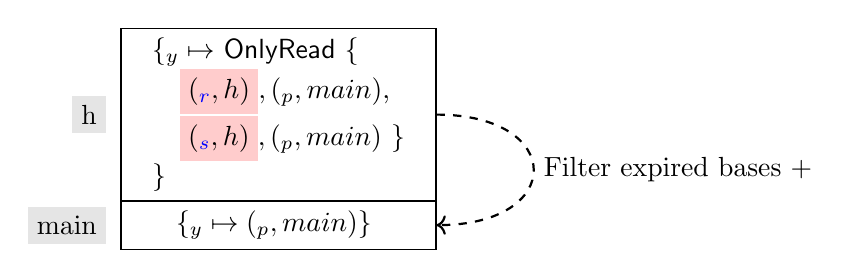
\begin{tikzpicture}[stack/.style={rectangle split, rectangle split parts=#1, draw, anchor=center, text centered,align=left},
    scope/.style={fill=gray!20, anchor=center}]
\node[stack=2, minimum width=4.0cm] (s) {
\nodepart[align=left]{one} \{$\Blockvar_y \mapsto$ $\mathsf{OnlyRead}$ \{ \\
                            \quad $\set{\text{\colorbox{red!20}{$(\Blockvar_\text{\textcolor{blue}{$r$}}, \scope{h})$}}, (\Blockvar_p, \scope{main})}$, \\
                            \quad $\set{\text{\colorbox{red!20}{$(\Blockvar_\text{\textcolor{blue}{$s$}}, \scope{h})$}}, (\Blockvar_p, \scope{main})}$ \} \\ \}
                
               
\nodepart{two} \{$\Blockvar_y \mapsto \restricted{\set{(\Blockvar_p, \scope{main})}}$\}
};
\node[scope, left=5pt of s.one west]   {\scope{h}};
\node[scope, left=5pt of s.two west]   {\scope{main}};

\draw[->, dashed, thick] (s.one east) to[bend left=90, looseness=3] node[right] {Filter expired bases + $\joinsym$} (s.two east);


\end{tikzpicture}

\leavevmode \\

\begin{itemize}
    \item Filtered state: $\onlyread{\set{\set{(\Blockvar_p, \scope{main})}}}$
    \item $\onlyread{\set{\set{(\Blockvar_p, \scope{main})}}} \joinsym \restricted{\set{(\Blockvar_p, \scope{main})}} = ...$
\end{itemize}

\end{frame}

% ---- 


\begin{frame}[fragile]
\frametitle{Aliasing loads (TMU)}
\centering
\colorbox{red!20}{$\onlyread{\set{\set{(\Blockvar_p, \scope{main})}}} \joinsym \restricted{\set{(\Blockvar_p, \scope{main})}} = \restricted{\set{(\Blockvar_p, \scope{main})}}$}
\\

\begin{minipage}{.43\textwidth}
\begin{itemize}
    \item The updated symmetric \joinsym \ operation (simplified)
    \item $\Basesvar \neq \Basesvar'$
\end{itemize}
\end{minipage}%
\begin{minipage}{.57\textwidth}
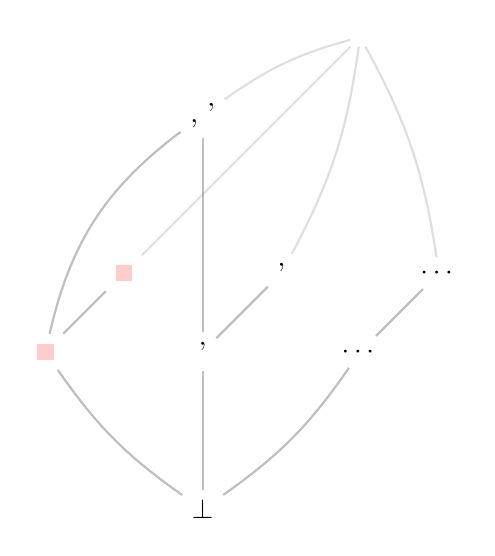
\begin{tikzpicture}
    \node (ub)     at (7,5) {\rsub};
    \node (un)     at (5,4) {\orabbr{\set{\Basesvar, \Basesvar'}}};
    \node (rsbs)   at (4,2) {\colorbox{red!20}{\resabbr{\Basesvar}}};
    \node (rsbs')  at (6,2) {\resabbr{\Basesvar'}};
    \node (rsbs'') at (8,2) {$\cdots$};
    \node (orbs)   at (3,1) {\colorbox{red!20}{\orabbr{\set{\Basesvar}}}};
    \node (orbs')  at (5,1) {\orabbr{\set{\Basesvar'}}};
    \node (orbs'') at (7,1) {$\cdots$};
    \node (bot)    at (5,-1) {$\bot$};

    \path[thick, black, opacity=0.25]
    (bot) edge[bend left=10] node {} (orbs)
    (bot) edge node {} (orbs')
    (bot) edge[bend right=10] node {} (orbs'')
    
    (orbs) edge node {} (rsbs) 
    (orbs') edge node {} (rsbs')
    (orbs'') edge node {} (rsbs'')  
    
    (orbs) edge[bend left=20] node {} (un)
    (orbs') edge node {} (un)
    % (orbs'') edge[bend right=20] node {} (un)

    (rsbs) edge[gray] node {} (ub)
    (rsbs') edge[bend right=10, gray] node {} (ub)
    (rsbs'') edge[bend right=10, gray] node {} (ub)

    (un) edge[bend left=10, gray] node {} (ub);
\end{tikzpicture}
\end{minipage}

\end{frame}


% ---- 


\begin{frame}[fragile]
\frametitle{Aliasing loads (TMU)}
\begin{itemize}
    \item Loads via aliased pointers are now permitted \smiley{}
    \item Achieved our goal of relaxing the semantics for this problem to give \textbf{less UB}, \textbf{consistent} with the ISO standard
\end{itemize}
\end{frame}


\begin{frame}
\frametitle{Crestrict refinements}
\begin{itemize}
\item Too much undefined behavior (TMU)
    \begin{itemize}
        \item[$\greentriangleright$] Aliasing loads: \textbf{adjust restrict states and $\joinsym$ lattice}
        \item Returning restrict pointers: \textbf{track active scopes and filter pointer values}
    \end{itemize}
\item Too little undefined behavior (TLU)
    \begin{itemize}
        \item Array of restrict pointers: \textbf{refine bases granularity to offsets}
        \item Nested restrict pointers: \textbf{missing subclause and pointer values as a tree structure}
        \item Semantic preservation under inlining: \textbf{deferred $\rightarrow$ eager check}
        \item Call to free: \textbf{update the restrict state}
    \end{itemize}
\end{itemize}

\begin{itemize}
    \item \textbf{Consistency}, goal 2 \cmark (\ie, to the best of our knowledge)
\end{itemize}

\end{frame}



\begin{frame}
\frametitle{Evaluation}
\begin{itemize}
    \item Implemented the semantics in an interpreter, written in Rust (\textbf{executable}, goal 3 \cmark)
    \item A (public) test suite dedicated to restrict does not exist
    \item Created our own suite of 96 tests, build around common restrict use cases and the discussed problems
\end{itemize}
\end{frame}



\begin{frame}
\frametitle{Conclusion}
\begin{itemize}
    \item Redeveloped the restrict fragment of the \cink semantics in a functional style (4)
    \item We argued it has six consistency problems
    \item We proposed changes to the semantic domains and rules to solve them (2)
    \item The new Crestrict semantics (1,3) were implemented in an interpreter and evaluated under a more extensive test suite   
\end{itemize}

\begin{enumerate}
    \item \textcolor{ao}{Unambiguous: \cmark}
    \item \textcolor{ao}{Consistent: \cmark}
    \item \textcolor{ao}{Executable: \cmark}
    \item \textcolor{ao}{Suitable: \cmark}
\end{enumerate}

\end{frame}


\begin{frame}
\frametitle{Future work}
\begin{itemize}
    \item Assignments between restrict pointers
    \item A more complete language
    \item Proving optimizations correct (the sequal of goal 4)
    \item ...
\end{itemize}
\end{frame}



% EXTRA SLIDES


\begin{frame}
\frametitle{}
\end{frame}


\begin{frame}[fragile]
\frametitle{Returning restrict pointers (TMU)}

\begin{minted}[escapeinside=||,mathescape=true]{c}
int* as_mut_ptr(int* restrict v) {
    return v;
}
\end{minted}

\vspace*{-1cm}

\begin{figure}[!h]
\begin{minipage}[t]{.4\textwidth}

\begin{minted}[escapeinside=||,mathescape=true]{c}
int main() {
    int a;

    int* p = as_mut_ptr(&a);
    int* q = as_mut_ptr(&a);

    *p = 0;
    |\colorbox{red!20}{*q = 0;}|
}

\end{minted}
\end{minipage}%
\begin{minipage}{.6\textwidth}
\colorbox{red!20}{$\restricted{\set{(\Blockvar_{v2}, \scope{as\_mut\_ptr\_2})}} \joinsym$} \\
\colorbox{red!20}{$\restricted{\set{(\Blockvar_{v1}, \scope{as\_mut\_ptr\_1})}} = \rsub$} \\

\executionannotation
{
    \{$\Blockvar_a \mapsto 0$, \\
        \ $\Blockvar_p \mapsto \ptr{(\Blockvar_a, \set{(\Blockvar_{v1}, \scope{as\_mut\_ptr\_1})})}$, \\
        \ $\Blockvar_q \mapsto \ptr{(\Blockvar_a, \set{(\Blockvar_{v2}, \scope{as\_mut\_ptr\_2})})}$
    \}
    }
{
    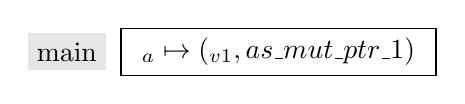
\begin{tikzpicture}[stack/.style={rectangle split, rectangle split parts=#1, draw, anchor=center, text centered},
        scope/.style={fill=gray!20, anchor=center}]
    \node[stack=1, minimum width=4.0cm] (s) {
        \nodepart{one} $\set{\Blockvar_a \mapsto \restricted{\set{(\Blockvar_{v1}, \scope{as\_mut\_ptr\_1})}}}$
    };

    \node[scope, left=5pt of s.one west]   {\scope{main}};
    

    \end{tikzpicture}
}
\end{minipage}
\end{figure}

\end{frame}



\begin{frame}[fragile]
\frametitle{Array of restrict pointers (TLU)}
\begin{minipage}{.45\textwidth}
\begin{minted}[escapeinside=||,mathescape=true]{c}
// Scope $\scope{main}$
int main() {
    int x;
    int* restrict a[2] = {&x, &x};

    *(a[0]) = 10;
    |\colorbox{red!20}{*(a[1]) = 11;}|
}
\end{minted}
\end{minipage}%
\begin{minipage}{.55\textwidth}
\colorbox{red!20}{$\restricted{\set{(\Blockvar_a, \scope{main})}} \joinsym \restricted{\set{(\Blockvar_a, \scope{main})}}$} \\
\colorbox{red!20}{$= \restricted{\set{(\Blockvar_a, \scope{main})}}$} \\

\executionannotation
{
    \{$\Blockvar_x \mapsto 10$, \\
      \ $\Blockvar_a \mapsto \{\ptr{(\Blockvar_x, \set{(\Blockvar_a, \scope{main})})}$,\\ 
      \ \qquad\quad $\ptr{(\Blockvar_x, \set{(\Blockvar_a, \scope{main})})}$ \}\}  
}
{
    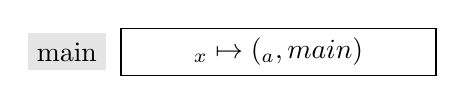
\begin{tikzpicture}[stack/.style={rectangle split, rectangle split parts=#1, draw, anchor=center, text centered},
        scope/.style={fill=gray!20, anchor=center}]
    \node[stack=1, minimum width=4.0cm] (s) {
        \nodepart{one} $\set{\Blockvar_x \mapsto \restricted{\set{(\Blockvar_a, \scope{main})}}}$
    };

    \node[scope, left=5pt of s.one west]   {\scope{main}};
    \end{tikzpicture}
}
\end{minipage}
\end{frame}


\begin{frame}[fragile]
\frametitle{Semantic preservation under inlining (TLU)}
\begin{minted}[escapeinside=||,mathescape=true]{c}
// Scope $\scope{foo}$
void foo(int* q) {
    *q = 0;
    |\colorbox{red!20}{while(1) \{\}}|
    // Never terminates
}
\end{minted}


\begin{minipage}{.4\textwidth}
\begin{minted}[escapeinside=||,mathescape=true]{c}
// Scope $\scope{main}$
int main() {
    int x = 5;
    int* restrict p = &x;
    *p;
    foo(&x);
}
\end{minted}
\end{minipage}%
\begin{minipage}{.6\textwidth}
\executionannotation
{
    \{$\Blockvar_x \mapsto 5$, \\
     \ $\Blockvar_p \mapsto \ptr{(\Blockvar_x, \set{(\Blockvar_p, \scope{main})})}$, \\
     \ $\Blockvar_q \mapsto \ptr{(\Blockvar_x, \emptyset)}$
    \}
}
{
    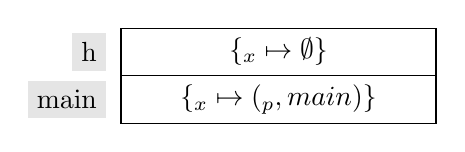
\begin{tikzpicture}[stack/.style={rectangle split, rectangle split parts=#1, draw, anchor=center, text centered},
        scope/.style={fill=gray!20, anchor=center}]
    \node[stack=2, minimum width=4.0cm] (s) {
    \nodepart{one} \{$\Blockvar_x \mapsto \restricted{\emptyset}$\}
    \nodepart{two} \{$\Blockvar_x \mapsto \onlyread{\set{(\Blockvar_p, \scope{main})}}$\}
    };
    \node[scope, left=5pt of s.one west]   {\scope{h}};
    \node[scope, left=5pt of s.two west]   {\scope{main}};
    \end{tikzpicture}
}
\end{minipage}

\end{frame}


\begin{frame}[fragile]
\frametitle{Semantic preservation under inlining (TLU)}
\begin{minipage}{.4\textwidth}
\begin{minted}[escapeinside=||,mathescape=true]{c}
// foo is inlined into main
// Scope $\scope{main}$
int main() {
    int x = 5;
    int* restrict p = &x;
    *p;
    int* q = &x;
    |\colorbox{red!20}{*q = 0;}|
    while (1) {}
}
\end{minted}
\end{minipage}%
\begin{minipage}{.6\textwidth}
\colorbox{red!20}{$\restricted{\emptyset} \joinsym \onlyread{\set{(\Blockvar_p, \scope{main})}} = \rsub$} \\

\executionannotation
{
    \{$\Blockvar_x \mapsto 5$, \\
     \ $\Blockvar_p \mapsto \ptr{(\Blockvar_x, \set{(\Blockvar_p, \scope{main})})}$, \\
     \ $\Blockvar_q \mapsto \ptr{(\Blockvar_x, \emptyset)}$
    \}
}
{
    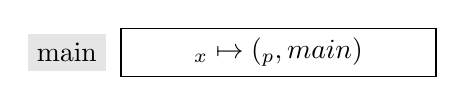
\begin{tikzpicture}[stack/.style={rectangle split, rectangle split parts=#1, draw, anchor=center, text centered},
        scope/.style={fill=gray!20, anchor=center}]
    \node[stack=1, minimum width=4.0cm] (s) {
        \nodepart{one} $\set{\Blockvar_x \mapsto \onlyread{\set{(\Blockvar_p, \scope{main})}}}$
    };

    \node[scope, left=5pt of s.one west]   {\scope{main}};
    \end{tikzpicture}
}
\end{minipage}

\end{frame}


\begin{frame}[fragile]
\frametitle{Call to free (TLU)}
\begin{minipage}{.5\textwidth}
\begin{minted}[escapeinside=||,mathescape=true]{c}
// Scope $\scope{bar}$
void bar(int* s) {
    free(s);
}
// Scope $\scope{foo}$
void foo(int* restrict q, int* r) {
    |\colorbox{red!20}{*q = 5;}|
    bar(r);
}
// Scope $\scope{main}$
int main() {
    // Stored at $\Blockvar_v$
    int* p = malloc(sizeof(int));
    foo(p, p);
}
\end{minted}
\end{minipage}%
\begin{minipage}{.5\textwidth}
\executionannotation
{
\{$\Blockvar_v \mapsto 5$, \\
   \ $\Blockvar_p \mapsto \ptr{(\Blockvar_v, \emptyset)}$, \\
    \ $\Blockvar_q \mapsto \ptr{(\Blockvar_v, \set{(\Blockvar_q, \scope{foo})})}$, \\
    \ $\Blockvar_r \mapsto \ptr{(\Blockvar_v, \emptyset)}$ \}
}
{
    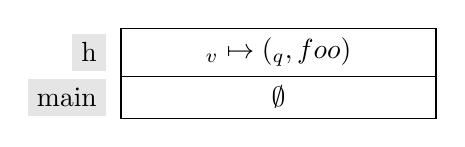
\begin{tikzpicture}[stack/.style={rectangle split, rectangle split parts=#1, draw, anchor=center, text centered},
        scope/.style={fill=gray!20, anchor=center}]
    \node[stack=2, minimum width=4.0cm] (s) {
    \nodepart{one} $\set{\Blockvar_v \mapsto \restricted{(\Blockvar_q, \scope{foo})}}$
    \nodepart{two} $\emptyset$
    };
    \node[scope, left=5pt of s.one west]   {\scope{h}};
    \node[scope, left=5pt of s.two west]   {\scope{main}};
    \end{tikzpicture}   
}
\end{minipage}

\end{frame}



\begin{frame}[fragile]
\frametitle{Nested restrict pointers (TLU)}
\begin{minipage}{0.7\textwidth}
\begin{minted}[escapeinside=||,mathescape=true,linenos]{c}
// Scope $\scope{foo}$
int foo(int *restrict *restrict p, int *restrict *restrict q) {
    **p = 10;
    **q = 11;
    return **p; // Optimized to 10 by GCC
}
// Scope $\scope{main}$
int main() {
    int x;
    int* xp = &x;
    foo(&xp, &xp);
}
\end{minted}
\end{minipage}%
\begin{minipage}[t]{0.3\textwidth}
\begin{tikzpicture}
    \node (pq) {\mintinline{c}{p,q}};
    \node[right of = pq] (xp) {\mintinline{c}{xp}};
    \node[right of = xp] (x) {\mintinline{c}{x}};

    \draw[->] (pq) -- (xp);
    \draw[->] (xp) -- (x);
\end{tikzpicture}
\end{minipage}

\begin{itemize}
    \item UB due to a subtle subclause of the standard
\end{itemize}

\end{frame}


% Restrict definition
\begin{frame}
\frametitle{Restrict definition (simplified)}
\begin{itemize}
    % \item A type qualifier for \textbf{pointer types}, \eg \mintinline{c}{int* restrict p;}
    \item A pointer is ``based on'' a restrict pointer if it depends on its value: \\
        \mintinline[mathescape=true]{c}{int x; int* restrict p = &x; int* q = p; // $q$ is based on $p$}  
    \item A \textbf{promise} from the programmer to the compiler that a restrict qualified pointer and pointers ``based on" it will \textbf{not alias} with other pointers during the \textbf{scope} it is alive if:
            \begin{itemize}
                \item The pointer is used to \textbf{access} the object it points to
                \item The object pointed to is \textbf{modified} (by any means)
            \end{itemize}
    \item \colorbox{red!20}{``Modifications of the object pointed to by a restrict pointer are considered to modify} \\ \colorbox{red!20}{the restrict pointer object itself"}
\end{itemize}
\end{frame}




\begin{frame}[fragile]
\frametitle{Nested restrict pointers (TLU)}
\begin{itemize}
    \item What does ``modifications of the object pointed to by a restrict pointer are considered to modify the restrict pointer object itself" mean?
    \item Modifications are represented by the restrict state $\restrictedn$
\end{itemize}

\pause

\begin{figure}[h]
\centering
\begin{minipage}{.5\textwidth}
\begin{minted}[escapeinside=||,mathescape=true]{c}
// Scope $\scope{main}$
{
int x; // $\&x = \Blockvar_x$
int* restrict p = &x; // $\&p = \Blockvar_p$
|\colorbox{red!20}{*p = 10;}| // Modification
}
\end{minted}
\end{minipage}%
\begin{minipage}{.5\textwidth}
\executionannotation
{
    \{$\Blockvar_x \mapsto \colorbox{red!20}{10}$, \\
      \ $\Blockvar_p \mapsto \ptr{(\Blockvar_x, \set{(\Blockvar_p, \scope{main})})}$
    \}
}
{
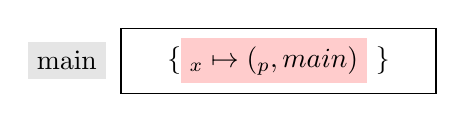
\begin{tikzpicture}[stack/.style={rectangle split, rectangle split parts=#1, draw, anchor=center, text centered},
    scope/.style={fill=gray!20, anchor=center}]

\node[stack=1, minimum width=4.0cm] (s) {
    \nodepart{one} \{\colorbox{red!20}{$\Blockvar_x \mapsto \restricted{\set{(\Blockvar_p, \scope{main})}}$} \}

};

\node[scope, left=5pt of s.one west]   {\scope{main}};

\end{tikzpicture}
}
\end{minipage}
\end{figure}


\end{frame}

\begin{frame}[fragile]
\frametitle{Nested restrict pointers (TLU)}
\begin{itemize}
    \item What does ``modifications of the object pointed to by a restrict pointer are considered to modify the restrict pointer object itself" mean?
    \item Modifications are represented by the restrict state \colorbox{blue!20}{$\restrictedn$}
\end{itemize}

\begin{figure}[h]
\centering
\begin{minipage}{.5\textwidth}
\begin{minted}[escapeinside=||,mathescape=true]{c}
// Scope $\scope{main}$
{
int x; // $\&x = \Blockvar_x$
int* restrict p = &x; // $\&p = \Blockvar_p$
|\colorbox{red!20}{*p = 10;}| // Modification
}
\end{minted}
\end{minipage}%
\begin{minipage}{.5\textwidth}
\executionannotation
{
    \{$\Blockvar_x \mapsto \colorbox{red!20}{10}$, \\
        \ $\Blockvar_p \mapsto \ptr{(\Blockvar_x, \set{(\Blockvar_p, \scope{main})})}$
    \}
}
{
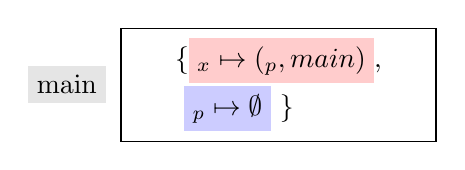
\begin{tikzpicture}[stack/.style={rectangle split, rectangle split parts=#1, draw, anchor=center, text centered},
    scope/.style={fill=gray!20, anchor=center}]

\node[stack=1, minimum width=4.0cm] (s) {
    \nodepart[align=left]{one} \{\colorbox{red!20}{$\Blockvar_x \mapsto \restricted{\set{(\Blockvar_p, \scope{main})}}$}, \\
                    \ \colorbox{blue!20}{$\Blockvar_p \mapsto \restricted{\emptyset} $} \}

};

\node[scope, left=5pt of s.one west]   {\scope{main}};

\end{tikzpicture}
}
\end{minipage}
\end{figure}


\end{frame}



\begin{frame}[fragile]
\frametitle{Nested restrict pointers (TLU)}
\begin{minted}[escapeinside=||,mathescape=true]{c}
// Scope $\scope{foo}$
int foo(int *restrict *restrict p, int *restrict *restrict q) {
    *|\colorbox{red!20}{*p}| = 10;
    **q = 11;
    return **p;
}
\end{minted}

\vspace*{-2cm}

\begin{figure}[!h]
\begin{minipage}[t]{.36\textwidth}
\begin{minted}[escapeinside=||,mathescape=true]{c}
// Scope $\scope{main}$
int main() {
    int x;
    int* xp = &x;
    foo(&xp, &xp);
}
\end{minted}
\end{minipage}%
\begin{minipage}{.64\textwidth}

\executionannotation
{
\{ $\Blockvar_x \mapsto \vundef$, \\
    \ $\Blockvar_{xp} \mapsto \ptr{(\Blockvar_x, \emptyset)}$, \\
    \ $\Blockvar_p \mapsto \ptr{(\Blockvar_{xp}, \set{(\Blockvar_p, \scope{foo})})}$, \\
    \ $\Blockvar_q \mapsto \ptr{(\Blockvar_{xp}, \set{(\Blockvar_q, \scope{foo})})}$ \}
}
{
    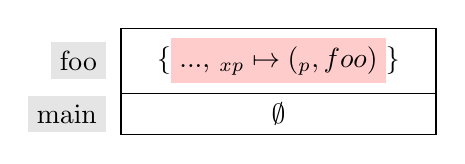
\begin{tikzpicture}[stack/.style={rectangle split, rectangle split parts=#1, draw, anchor=center, text centered},
        scope/.style={fill=gray!20, anchor=center}]
    \node[stack=2, minimum width=4.0cm] (s) {
    \nodepart{one} \{\colorbox{red!20}{..., $\Blockvar_{xp} \mapsto \onlyread{\set{(\Blockvar_p, \scope{foo})}}$}\}
    \nodepart{two} $\emptyset$
    };
    \node[scope, left=5pt of s.one west]   {\scope{foo}};
    \node[scope, left=5pt of s.two west]   {\scope{main}};
    \end{tikzpicture}   
}

\end{minipage}
\end{figure}


\end{frame}



\begin{frame}[fragile]
\frametitle{Nested restrict pointers (TLU)}
\begin{minted}[escapeinside=||,mathescape=true]{c}
// Scope $\scope{foo}$
int foo(int *restrict *restrict p, int *restrict *restrict q) {
    |\colorbox{red!20}{**p}| = 10;
    **q = 11;
    return **p;
}
\end{minted}

\vspace*{-2cm}

\begin{figure}[!h]
\begin{minipage}[t]{.36\textwidth}
\begin{minted}[escapeinside=||,mathescape=true]{c}
// Scope $\scope{main}$
int main() {
    int x;
    int* xp = &x;
    foo(&xp, &xp);
}
\end{minted}
\end{minipage}%
\begin{minipage}{.64\textwidth}

\executionannotation
{
\{ $\Blockvar_x \mapsto \vundef$, \\
    \ $\Blockvar_{xp} \mapsto \ptr{(\Blockvar_x, \emptyset)}$, \\
    \ $\Blockvar_p \mapsto \ptr{(\Blockvar_{xp}, \set{(\Blockvar_p, \scope{foo})})}$, \\
    \ $\Blockvar_q \mapsto \ptr{(\Blockvar_{xp}, \set{(\Blockvar_q, \scope{foo})})}$ \}
}
{
    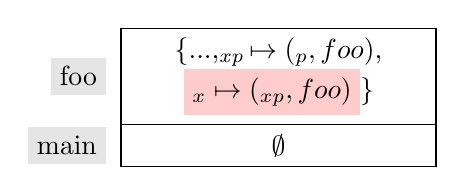
\begin{tikzpicture}[stack/.style={rectangle split, rectangle split parts=#1, draw, anchor=center, text centered},
        scope/.style={fill=gray!20, anchor=center}]
    \node[stack=2, minimum width=4.0cm] (s) {
    \nodepart[align=left]{one} \{$..., \Blockvar_{xp} \mapsto \onlyread{\set{(\Blockvar_p, \scope{foo})}}$, \\
                     \ \colorbox{red!20}{$\Blockvar_x \mapsto \restricted{\set{(\Blockvar_{xp}, \scope{foo})}}$}\}
    \nodepart{two} $\emptyset$
    };
    \node[scope, left=5pt of s.one west]   {\scope{foo}};
    \node[scope, left=5pt of s.two west]   {\scope{main}};
    \end{tikzpicture}   
}

\end{minipage}
\end{figure}

\end{frame}


\begin{frame}[fragile]
\frametitle{Nested restrict pointers (TLU)}

\begin{itemize}
    \item We now need to change the restrict state of $\Blockvar_{xp}$ to $\restrictedn$
    \item The only $\restrictedn$ state joinable with the current state is \colorbox{blue!20}{$\restricted{\set{(\Blockvar_p, \scope{foo})}}$}
    \item Problem: \textbf{not enough information} to produce this state, \ie the semantics did a store through $\ptr{(\Blockvar_x, \set{(\Blockvar_{xp}, \scope{foo})})}$
\end{itemize}

\leavevmode \\

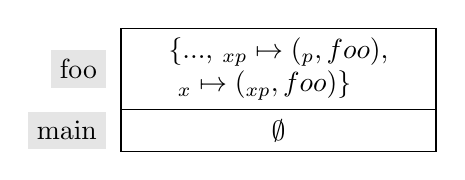
\begin{tikzpicture}[stack/.style={rectangle split, rectangle split parts=#1, draw, anchor=center, text centered},
    scope/.style={fill=gray!20, anchor=center}]
\node[stack=2, minimum width=4.0cm] (s) {
\nodepart[align=left]{one} \{..., $\Blockvar_{xp} \mapsto \onlyread{\set{(\Blockvar_p, \scope{foo})}}$, \\
                 \ $\Blockvar_x \mapsto \restricted{\set{(\Blockvar_{xp}, \scope{foo})}}$\}
\nodepart{two} $\emptyset$
};
\node[scope, left=5pt of s.one west]   {\scope{foo}};
\node[scope, left=5pt of s.two west]   {\scope{main}};
\end{tikzpicture}

\end{frame}


\begin{frame}
\frametitle{Nested restrict pointers (TLU)}

\begin{itemize}
    \item Idea: pointer value as a \textbf{tree} structure, to track how bases themselves are derived!
    \item $\ptr{(\Blockvar_x, \set{((\Blockvar_{xp}, \set{((\Blockvar_p, \emptyset), \scope{foo})}), \scope{foo})})}$ \\~\\
    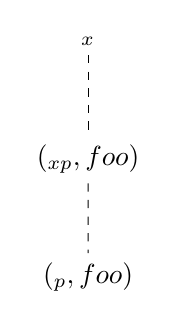
\begin{tikzpicture}[sibling distance=25mm,      edge from parent/.style={draw, dashed},
        every edge/.append style={->}    ]
    \node (root) {$\Blockvar_x$}
        child {node {$(\Blockvar_{xp}, \scope{foo})$}
        child {node {$(\Blockvar_p, \scope{foo})$}}
        };
    
    \end{tikzpicture}

\end{itemize}
    
\end{frame}



\begin{frame}[fragile]
\frametitle{Nested restrict pointers (TLU)}
\begin{minted}[escapeinside=||,mathescape=true]{c}
// Scope $\scope{foo}$
int foo(int *restrict *restrict p, int *restrict *restrict q) {
    |\colorbox{red!20}{**p}| = 10;
    **q = 11;
    return **p;
}
\end{minted}

\vspace*{-2cm}

\begin{figure}[!h]
\begin{minipage}[t]{.3\textwidth}
\begin{minted}[escapeinside=||,mathescape=true]{c}
// Scope $\scope{main}$
int main() {
    int x;
    int* xp = &x;
    foo(&xp, &xp);
}
\end{minted}
\end{minipage}%
\begin{minipage}{.7\textwidth}

\executionannotation
{
\{ $\Blockvar_x \mapsto \vundef$, \\
    \ $\Blockvar_{xp} \mapsto \ptr{(\Blockvar_x, \emptyset)}$, \\
    \ $\Blockvar_p \mapsto \ptr{(\Blockvar_{xp}, \set{((\Blockvar_p, \emptyset), \scope{foo})})}$, \\
    \ $\Blockvar_q \mapsto \ptr{(\Blockvar_{xp}, \set{((\Blockvar_q, \emptyset), \scope{foo})})}$ \}
}
{
    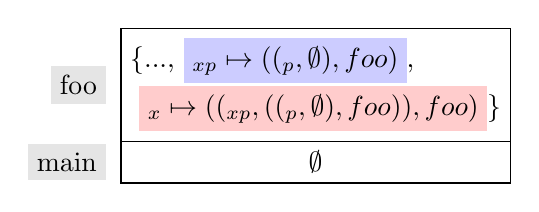
\begin{tikzpicture}[stack/.style={rectangle split, rectangle split parts=#1, draw, anchor=center, text centered},
        scope/.style={fill=gray!20, anchor=center}]
    \node[stack=2, minimum width=4.0cm] (s) {
    \nodepart[align=left]{one} \{..., \colorbox{blue!20}{$\Blockvar_{xp} \mapsto \restricted{\set{((\Blockvar_p, \emptyset), \scope{foo})}}$}, \\
                        \ \colorbox{red!20}{$\Blockvar_x \mapsto \restricted{\set{((\Blockvar_{xp}, \set{((\Blockvar_p, \emptyset), \scope{foo})}), \scope{foo})}}$}\}
    \nodepart{two} $\emptyset$
    };
    \node[scope, left=5pt of s.one west]   {\scope{foo}};
    \node[scope, left=5pt of s.two west]   {\scope{main}};
    \end{tikzpicture}   
}

\end{minipage}
\end{figure}

\end{frame}



\begin{frame}[fragile]
\frametitle{Nested restrict pointers (TLU)}
\begin{minted}[escapeinside=||,mathescape=true]{c}
// Scope $\scope{foo}$
int foo(int *restrict *restrict p, int *restrict *restrict q) {
    **p = 10;
    *|\colorbox{red!20}{*q}| = 11;
    return **p;
}
\end{minted}

\vspace*{-2cm}

\begin{figure}[!h]
\begin{minipage}[t]{.3\textwidth}
\begin{minted}[escapeinside=||,mathescape=true]{c}
// Scope $\scope{main}$
int main() {
    int x;
    int* xp = &x;
    foo(&xp, &xp);
}
\end{minted}
\end{minipage}%
\begin{minipage}{.7\textwidth}

\executionannotation
{
\{ $\Blockvar_x \mapsto \vundef$, \\
    \ $\Blockvar_{xp} \mapsto \ptr{(\Blockvar_x, \emptyset)}$, \\
    \ $\Blockvar_p \mapsto \ptr{(\Blockvar_{xp}, \set{((\Blockvar_p, \emptyset), \scope{foo})})}$, \\
    \ $\Blockvar_q \mapsto \ptr{(\Blockvar_{xp}, \set{((\Blockvar_q, \emptyset), \scope{foo})})}$ \}
}
{
    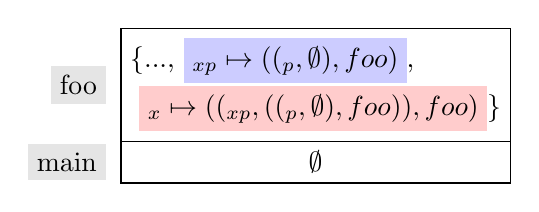
\begin{tikzpicture}[stack/.style={rectangle split, rectangle split parts=#1, draw, anchor=center, text centered},
        scope/.style={fill=gray!20, anchor=center}]
    \node[stack=2, minimum width=4.0cm] (s) {
    \nodepart[align=left]{one} \{..., \colorbox{blue!20}{$\Blockvar_{xp} \mapsto \restricted{\set{((\Blockvar_p, \emptyset), \scope{foo})}}$}, \\
                        \ \colorbox{red!20}{$\Blockvar_x \mapsto \restricted{\set{((\Blockvar_{xp}, \set{((\Blockvar_p, \emptyset), \scope{foo})}), \scope{foo})}}$}\}
    \nodepart{two} $\emptyset$
    };
    \node[scope, left=5pt of s.one west]   {\scope{foo}};
    \node[scope, left=5pt of s.two west]   {\scope{main}};
    \end{tikzpicture}   
}

\end{minipage}
\end{figure}

\end{frame}



\begin{frame}[fragile]
\frametitle{Nested restrict pointers (TLU)}
\begin{minted}[escapeinside=||,mathescape=true]{c}
// Scope $\scope{foo}$
int foo(int *restrict *restrict p, int *restrict *restrict q) {
    **p = 10;
    *|\colorbox{red!20}{*q}| = 11;
    return **p;
}
\end{minted}

\vspace*{-2cm}

\begin{figure}[!h]
\begin{minipage}[t]{.3\textwidth}
\begin{minted}[escapeinside=||,mathescape=true]{c}
// Scope $\scope{main}$
int main() {
    int x;
    int* xp = &x;
    foo(&xp, &xp);
}
\end{minted}
\end{minipage}%
\begin{minipage}{.7\textwidth}
\colorbox{red!20}{$\onlyread{\set{((\Blockvar_\text{\textcolor{blue}{$q$}}, \emptyset), \scope{foo})}} \joinsym  \restricted{\set{((\Blockvar_\text{\textcolor{blue}{$p$}}, \emptyset), \scope{foo})}} = ...$} \\

\executionannotation
{
\{ ..., \\
    \ $\Blockvar_q \mapsto \ptr{(\Blockvar_{xp}, \set{((\Blockvar_q, \emptyset), \scope{foo})})}$ \}
}
{
    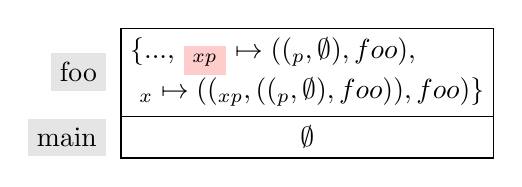
\begin{tikzpicture}[stack/.style={rectangle split, rectangle split parts=#1, draw, anchor=center, text centered},
        scope/.style={fill=gray!20, anchor=center}]
    \node[stack=2, minimum width=4.0cm] (s) {
    \nodepart[align=left]{one} \{..., \colorbox{red!20}{$\Blockvar_{xp}$} $\mapsto \restricted{\set{((\Blockvar_p, \emptyset), \scope{foo})}}$, \\
                        \ $\Blockvar_x \mapsto \restricted{\set{((\Blockvar_{xp}, \set{((\Blockvar_p, \emptyset), \scope{foo})}), \scope{foo})}}$\}
    \nodepart{two} $\emptyset$
    };
    \node[scope, left=5pt of s.one west]   {\scope{foo}};
    \node[scope, left=5pt of s.two west]   {\scope{main}};
    \end{tikzpicture}   
}

\end{minipage}
\end{figure}

\end{frame}






\begin{frame}[fragile]
\frametitle{Nested restrict pointers (TLU)}
\centering
\colorbox{red!20}{$\onlyread{\set{((\Blockvar_\text{\textcolor{blue}{$q$}}, \emptyset), \scope{foo})}} \joinsym  \restricted{\set{((\Blockvar_\text{\textcolor{blue}{$p$}}, \emptyset), \scope{foo})}} = \rsub$} \\

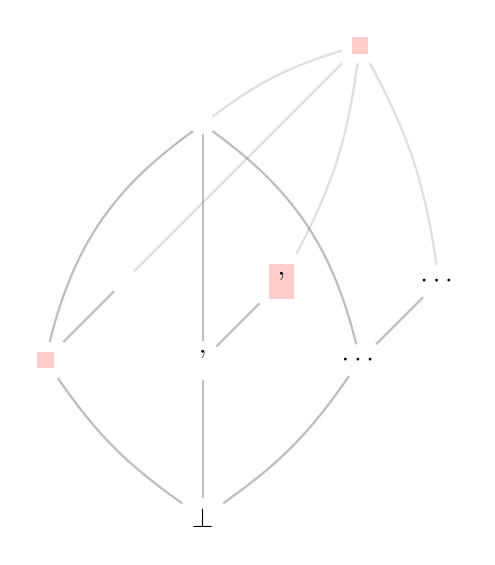
\begin{tikzpicture}
    \node (ub)     at (7,5) {\colorbox{red!20}{\rsub}};
    \node (un)     at (5,4) {\unresabbr};
    \node (rsbs)   at (4,2) {\resabbr{\Basesvar}};
    \node (rsbs')  at (6,2) {\colorbox{red!20}{\resabbr{\Basesvar'}}};
    \node (rsbs'') at (8,2) {$\cdots$};
    \node (orbs)   at (3,1) {\colorbox{red!20}{\orabbr{\Basesvar}}};
    \node (orbs')  at (5,1) {\orabbr{\Basesvar'}};
    \node (orbs'') at (7,1) {$\cdots$};
    \node (bot)    at (5,-1) {$\bot$};

    \path[thick, black, opacity=0.25]
    (bot) edge[bend left=10] node {} (orbs)
    (bot) edge node {} (orbs')
    (bot) edge[bend right=10] node {} (orbs'')
    
    (orbs) edge node {} (rsbs) 
    (orbs') edge node {} (rsbs')
    (orbs'') edge node {} (rsbs'')  
    
    (orbs) edge[bend left=20] node {} (un)
    (orbs') edge node {} (un)
    (orbs'') edge[bend right=20] node {} (un)

    (rsbs) edge[gray] node {} (ub)
    (rsbs') edge[bend right=10, gray] node {} (ub)
    (rsbs'') edge[bend right=10, gray] node {} (ub)

    (un) edge[bend left=10, gray] node {} (ub);
\end{tikzpicture}

\end{frame}


\begin{frame}[fragile]
\frametitle{Nested restrict pointers (TLU)}
\begin{itemize}
    \item Implemented a subtle subclause of the standard (in line with the GCC interpretation)
    \begin{itemize}    
        \item Updated pointer values to a \textbf{tree-like structure} to track how bases themselves are derived
    \end{itemize}
    \item Achieved our goal of giving undefined behavior \smiley{}
\end{itemize}

\end{frame}


\begin{frame}[fragile]
    \frametitle{Where are bases added to the pointer value?}

\begin{minted}[escapeinside=||,mathescape=true]{c}
// Scope $\scope{main}$
{
    int x; // $\&x = \Blockvar_x$
    int* restrict p = &x; // $\& \Blockvar_p$

    int* q = p; // Propagate the bases to q
    *p = ...;   // Used directly in lvalue position 
}
\end{minted}
{
\hspace*{-10pt}
\scriptsize
\begin{prooftree}
\AxiomC{$E(p) = \Blockvar_p$}
\RightLabel{\scriptsize{(EId)}}
\UnaryInfC{$\GEJudgment p, \Statevar \lval \colorbox{red!20}{$(\Blockvar_p, \emptyset)$}, \Statevar'$}

\AxiomC{$(\textcode{load} \ \Statevar' \ (\Blockvar_p, \emptyset)) = \ptr{(\Blockvar_x, \emptyset)}, \Statevar''$}

\AxiomC{$\isrestrict{e}$}

\RightLabel{\colorbox{red!20}{\scriptsize(ELvalConvRestrict)}}
\TrinaryInfC{$\GEJudgment p, \Statevar \rval \textcode{add\_prov} \ (\ptr{(\Blockvar_x, \emptyset)}) \ \colorbox{red!20}{$((\Blockvar_p, \emptyset), \scope{main})$}, \Statevar'' $}

% \RightLabel{\colorbox{red!20}{\scriptsize(Reduction)}}
% \UnaryInfC{$\GEJudgment p \rval \ptr{(\Blockvar_x, \set{((\Blockvar_p, \emptyset), \scope{main})})} $}

\RightLabel{\scriptsize(EDeref)}
\UnaryInfC{$\GEJudgment *p, \Statevar \lval (\Blockvar_x, \set{\colorbox{red!20}{$((\Blockvar_p, \emptyset), \scope{main})$}}), \Statevar''$}

\end{prooftree}
}
% \UnaryInfC{$p \lval l_1$}
% \AxiomC{$M(l_1) = \ptr{l_2}$}
% \RightLabel{\scriptsize(LValConv)}

% \BinaryInfC{$p \rval \ptr{l_2}$}
% \RightLabel{\scriptsize(EDeref)}

% \UnaryInfC{$*p \lval l_2$}
% \AxiomC{$M(l_2) = \ptr{l_3}$}
% \RightLabel{\scriptsize(LValConv)}

% \BinaryInfC{$\redm{*p \rval \ptr{l_3}}$}
% \RightLabel{\scriptsize(EDeref)}

% % \UnaryInfC{$\mathbin{**}p \lval l_3$}
% \end{prooftree}

\end{frame}





\end{document}
